%Version 3.1 December 2024
% Structured for Overleaf using sn-jnl, following the same conventions as the
% MIMIC-MJX manuscript template. Figures are left as placeholder \includegraphics
% calls pointing at figs/fig1.pdf ... figs/fig6.pdf -- swap in the real PDFs later.
%
%%%%%%%%%%%%%%%%%%%%%%%%%%%%%%%%%%%%%%%%%%%%%%%%%%%%%%%%%%%%%%%%%%%%%%
%% Submit your LaTeX manuscript as one .tex document.                %%
%% All additional figures/files should be attached separately and    %%
%% not embedded in the \TeX\ document itself.                        %%
%%%%%%%%%%%%%%%%%%%%%%%%%%%%%%%%%%%%%%%%%%%%%%%%%%%%%%%%%%%%%%%%%%%%%%

\documentclass[pdflatex, sn-nature]{sn-jnl}
% Center the text block on each page (avoids the twoside binding-offset shift)
% Also increase \footskip so page numbers don't collide with bottom floats/captions.
\geometry{hcentering,bindingoffset=0mm,footskip=150pt}

%%%% Standard Packages
\usepackage{graphicx}%
\usepackage{multirow}%
\usepackage{amsmath,amssymb,amsfonts}%
\usepackage{amsthm}%
\usepackage{mathrsfs}%
\usepackage[title]{appendix}%
\usepackage{xcolor}%
\usepackage{textcomp}%
\usepackage{manyfoot}%
\usepackage{float}%
\usepackage{placeins}%  % \FloatBarrier, keeps floats within their section
\renewcommand{\topfraction}{0.9}%
\renewcommand{\bottomfraction}{0.8}%
\renewcommand{\textfraction}{0.07}%
\renewcommand{\floatpagefraction}{0.7}%
\setcounter{topnumber}{2}%
\setcounter{bottomnumber}{2}%
\setcounter{totalnumber}{4}%
\usepackage{bm}%
\usepackage{booktabs}%
\usepackage{algorithm}%
\usepackage{algorithmicx}%
\usepackage{algpseudocode}%
\usepackage{listings}%
\usepackage{caption}
\usepackage{tabularx}
\usepackage{makecell}
\usepackage{array}
\usepackage{amsmath}
\usepackage[mathlines]{lineno}   

\captionsetup{font=footnotesize}

\theoremstyle{thmstyleone}%
\newtheorem{theorem}{Theorem}%
\newtheorem{proposition}[theorem]{Proposition}%

\theoremstyle{thmstyletwo}%
\newtheorem{example}{Example}%
\newtheorem{remark}{Remark}%

\theoremstyle{thmstylethree}%
\newtheorem{definition}{Definition}%

\raggedbottom

\begin{document}
\linenumbers

\title[Article Title]{LUC3D: Browser-based 3D annotation and proofreading GUI for pose estimation and multi-animal tracking}

%%=============================================================%%
%% GivenName -> \fnm{}   Particle -> \spfx{}   FamilyName -> \sur{}
%%=============================================================%%

\author[1]{\fnm{Eric} \spfx{J.} \sur{Leonardis}}
\author[2]{\fnm{Stefan} \spfx{N.} \sur{Oline}}
\author[1]{\fnm{Isaac} \sur{Tang}}
\author[1]{\fnm{Joshua} \sur{Park}}
\author[2]{\fnm{Bartul} \sur{Mimica}}
\author[1]{\fnm{Liezl} \sur{Maree}}
\author[2,1]{\fnm{Shayan} \sur{Afshar}}
\author[1]{\fnm{Aaron} \sur{Zhu}}
\author[1]{\fnm{Talisa} \sur{Wines}}
\author[1]{\fnm{Kay} \spfx{M.} \sur{Tye}}
\author[2]{\fnm{Mala} \sur{Murthy}}
\author[2]{\fnm{Annegret} \spfx{L.}  \sur{Falkner}}
\author*[1]{\fnm{Talmo} \spfx{D.} \sur{Pereira}}\email{talmo@salk.edu}

\affil[1]{\orgname{Salk Institute for Biological Studies}, \orgaddress{\city{La Jolla}, \state{CA}, \country{USA}}}
\affil[2]{\orgname{Princeton Neuroscience Institute, Princeton University}, \orgaddress{\city{Princeton}, \state{NJ}, \country{USA}}}

% max 150 words, unreferenced
\abstract{Animal behavior unfolds in three dimensions over time, yet accessible scientific tools for analyzing it in its natural form remain limited. Uncertainty from popular 2D pose methods can be refined with multi-camera approaches to produce more accurate 3D estimates. This paper presents LUC3D (Label Unification and Correspondence in 3D Annotation GUI), a browser-based 3D GUI for reducing the amount of manual labor required for labeling, proofreading, and multi-camera multi-animal tracking while requiring no installation to maximize accessibility. As proof-of-concept we present two datasets of proofread multi-camera 3D triangulated pose data of mouse social behavior, a protocol for generating 3D consistent labels, and a cross-view ReID tracking algorithm for multi-animal multi-camera pose data. This tool allows for the widespread adoption of 3D pose estimation techniques for studying social behavior while reducing the cost of entry for neuroscience labs across the world.}

\maketitle

\section{Introduction}\label{sec1}

Advances in deep learning for 2D pose estimation in humans have led to the development of accessible and popular methods for quantifying animal behavior \citep{Mathis2018,Pereira2020,Pereira2022,Biderman2024}. The human pose estimation literature has demonstrated that the solution to the problems caused by the limitations of 2D is to use multiple camera views to enable 3D pose estimation \citep{Iskakov2019}. This methodology has been applied to 3D pose estimation of animal behavior \citep{Dunn2021,Karashchuk2021}. Anipose in particular \citep{Karashchuk2021} has become a widely used and reliable tool for camera calibration and triangulation but, as a Python package that must be installed and run from the command line, requires technical expertise. Specialized tools have also been created for tracking the 3D movement of the face in rodents \citep{Daruwalla2026}. These single-subject 3D methods have since been extended to enable 3D pose estimation of multiple individuals simultaneously \citep{Huang2020,Chen2020}, a methodology that has similarly been extended to multi-animal applications \citep{Marshall2021,Marshall2022}. While other 3D annotation GUIs exist, they often involve a non-trivial installation process \citep{Hueser2023}. Recently, LightningPose3D was developed for multi-view 3D pose estimation and labeling in the browser, though it still requires a local installation \citep{Aharon2026}. Despite this progress there are still gaps in accessibility and integration. 3D pose estimation remains out of reach for labs without the resources to install and maintain these tools. Even where it is available the workflow is fragmented across separate packages for calibration, labeling, cross-view identification and proofreading. Progress is further limited by the lack of large benchmark datasets of multiple animals in enriched environments with heavy occlusion.

Here we present LUC3D, a browser-based GUI that builds on SLEAP's 2D pose tools to provide 3D-consistent cross-view labeling, tracking, and proofreading with no installation required. LUC3D relies on triangulation which recovers a 3D point from its 2D detections in multiple views and reprojection which projects that 3D point back into each camera's 2D view. Reprojections let users label a subset of views and correct the rest, which speeds up multi-view labeling considerably. LUC3D also includes a cross-view tracker that uses 3D geometry to identify the same animal across cameras \citep{Maree2024}, and a browser-based camera calibration tool, making 3D pose estimation possible without leaving the browser.

Several practical issues make 3D multi-animal pose estimation harder to adopt than single-camera methods. Building a multi-camera training set can be costly, since single-camera pose estimation methods require many manually labeled frames per view before a model performs reliably. Reprojection-aided labeling lets a frame labeled in a few anchor views generate accurate labels in all remaining views, sharply reducing the number of manual labels needed to generate a consistent training set. Proofreading requires resolving identity separately within each view before identity can be linked across views. The LUC3D cross-view tracker resolves identity across all cameras at once, so proofreading a session requires reviewing it once rather than once per camera. Adding more cameras also gives the tracker more redundant evidence for improving identity estimates. This paper provides a browser-based 3D annotation, proofreading, tracking, and calibration interface that makes 3D multi-animal pose estimation more usable and accessible. We also provide two challenging benchmark datasets for future 3D cross-view tracking methods.

This paper presents two comprehensive datasets: Mouse-Dyad-10M, with two mice per session, and SLAP-2M, with up to four mice and multiple levels of environmental enrichment. Many popular 2D datasets lack environmental enrichment because they introduce occlusions at the cost of limiting naturalism and experimental scope. SLAP-2M contains different levels of enrichment, demonstrating that with 3D pose estimation, enrichment and good tracking need not be mutually exclusive. As such, this dataset is well suited for benchmarking new models for behavioral segmentation and 3D pose estimation because its difficulty varies with the number of enrichment objects and the number of animals.


\section{Results}\label{sec2}

\subsection{A browser-based tool that speeds up annotation and resolves cross-view identity}\label{subsec2-1}

Multi-camera pose recording introduces the problem of linking identities across views, in addition to the single-camera problem of linking them across frames. Figure~\ref{fig1}A shows two multi-view recording setups: the SLAP-2M cage with eight cameras and up to 4 animals and the Mouse-Dyad-10M arena with five cameras and 2 animals (rendered from a single session's own calibration and tracked 3D poses). The single-camera problems of finding the keypoints in each view and tracking them across frames are solved by existing detectors and proofreading tools. The multi-camera problem of cross-view identification, deciding which detection in one view is the same animal in another, currently has no standard tool, limiting 3D reconstruction and proofreading. Cross-view ID has been traditionally solved either by manual assignment, or assuming that the initial tracks have no dropped frames \citep{Klibaite2025, Waldmann2024}. Here we build on the 2D pose tools from SLEAP \citep{Pereira2022} to address the three downstream stages: cross-view re-identification, triangulation, and proofreading of the resulting 3D poses.

LUC3D addresses the problems presented by multi-camera 3D annotation and tracking in a web browser, with no installation and no build step required (Figure~\ref{fig1}B). LUC3D does not include a detector, but is specifically designed to easily load and export SLEAP predictions. Figure~\ref{fig1}C shows the operation on a single frame of an eight-camera recording of three mice. The detector supplies 25 detections across the eight views with 21 distinct track names. Those names are per camera and arbitrary, for example the same animal is track 89 in one view (Camera 0) and track 83 in another (Camera 7). After re-identification the frame contains three identities, one per animal in every view, with 24 of the 25 detections assigned, such that all tracks associated with the aforementioned animal's are assigned to ID 1 (Figure~\ref{fig1}C, \textit{right}). Importantly, LUC3D identifies that the remaining detection is a duplicate of an already-matched animal in a view the panel does not show, which one-to-one assignment correctly refuses. In Figure~\ref{fig1}D, we next show how LUC3D triangulates that frame and fills all 45 of its 3D keypoints, shown beside the 2D detections in one camera (\textit{left}) so that it can be compared directly with that camera's video. Figure~\ref{fig1}E compared LUC3D to existing packages designed to address similar issues, notably Label3D and JARVIS both provide it \citep{Hueser2023, Aldarondo2019}. However, no other tool combines annotation-time cross-view identity, multi-animal support, a 3D proofreading viewport, all running in a browser without installation.

\begin{figure}[p]
  \centering
  % Keep this figure+caption away from the footer/page number region.
\includegraphics[width=1.0\textwidth,height=1.0\textheight,keepaspectratio]{figs/fig1.pdf}
  \caption{\textbf{LUC3D annotates and proofreads multi-camera 3D pose in a browser with no installation, and assigns cross-view identity} \textbf{A}, The SLAP-2M rig, left: 8 calibrated cameras and the cage with the tracked 3D poses of four animals. The Mouse-Dyad-10M rig, right: the 5 calibrated cameras and enclosure with tracked 3D poses of the two animals. \textbf{B}, Pipeline of a standard recording and labelling session. Video acquisition, 2D pose estimation (SLEAP or any other predictor as .slp), cameras are calibrated with a browser-based tool, cross-view re-identification, one per animal; triangulation collapses the tiles into a single 3D volume which is then proofread against per-view reprojections; and the project exports as .slp 2.8 or HDF5. The bracket marks the stages contributed by this paper. \textbf{C}, Cross-view re-identification on one frame of an 8-camera, 3-mouse recording with a 15-node skeleton. The four tiles are the same two views, cam 0 mid (far left) and cam 7 sideR (left), before and after. The per-camera tracks supplied to the app, each labeled with the track name its own camera assigned. Then the same two views after re-identification, each labeled with the resolved identity (right and far right). Track colors are arbitrary, so the same animal is a different color and a different track name in the two views on the left. Identity colors are shared by every view, so each animal keeps one color and one number in both views on the right. \textbf{D}, The same frame triangulated into 3D. Left, cam 0 mid with identity overlays. Middle, the 3D viewport. Right, the rig with 7 of the 8 calibrated cameras (cam 3 sideC, far from the others, is omitted for framing), 3 animals and 45 keypoints. \textbf{E}, Capability comparison against 7 multi-animal or multi-camera pose tools, read from each tool's published documentation. A dash means the capability is not documented or not applicable.}

  \label{fig1}
\end{figure}

\subsection{Reprojection from two labeled views reduces manual annotation}\label{subsec2-2}

Traditional manual multi-camera annotation scales linearly with the number of cameras, such that using two cameras requires twice as much time spent labeling frames, especially when each camera view observes the animal and enclosure from a different perspective. To generate a training set of 2D labeled frames, the user had to label frames from each camera view independently, manually placing all keypoints across all views, meaning that each additional camera added to a rig requires that the user generate another set of labeled frames for that view. Additionally, keypoints that were not visible in the current view required the user to provide their best guess. However, since as few as only two views is sufficient to project a point into 3D space (Figure~\ref{fig2}A,1-2), using LUC3D the user can rotate from one view to the next, labeling only confident keypoints. Remaining views inherit the placement of any unlabeled keypoints via reprojection of the 3D point back onto the unlabeled view (Figure~\ref{fig2}A3), such that the user can move from view to view, only labeling keypoints they are confident in placing, and correcting those reprojections that lack good correspondence to the animals in the video (Figure~\ref{fig2}A4). Therefore, when using reprojection-aided labeling, adding additional cameras to an experimental preparation can drastically save the user time when labeling frames, while increasing the precision of each keypoint's placement. 

Figure~\ref{fig2}B compares the number of mouse clicks between manual labeling and reprojection-aided labeling. On the measured five-camera rig, accepting reprojections at 10 pixels reduces manual placements from 75 per animal to 32, a 2.3-fold reduction in manual labeling. Modifying those reprojections would result in 48 placements per animal, which is a 1.6-fold reduction in manual labeling and would reduce the error to $\sim$5 pixels. The saved labor grows with rig size because the labeled two views can reproject to any number of remaining cameras. This estimates the labeling effort saved by using reprojections in the labeling process. This assumes that each node would be manipulated separately, but the GUI provides methods for translating the points for one animal in a view (hereafter referred to as an ``instance'') which can also reduce labeling time. 

The relationship between the numbers of cameras used in triangulation and the 3D error demonstrates that multi-view geometry reduces the uncertainty of pose estimates. A 3D point solved from two views is a median 4.74~mm from the reference, and the full five-view solve is 1.19~mm from it (Figure~\ref{fig2}C). The reference is the proofread 3D reconstruction, which was itself solved from all five views and then corrected by hand. The value at five cameras therefore measures the size of the proofreading corrections, and the values at fewer cameras are relative to it. The out-of-sample measurement, the error in a camera left out of the solve, is in Figure~\ref{fig2}E. 

The cost of solving from only two views depends on where those two cameras are placed relative to each other (See Figure~\ref{fig2}D). Error falls as $k$ over the sine of the angle between the two cameras relative to the animal (dashed curve). For example, the narrowest angle pair at 13 degrees gives 12.6~mm of error while the widest at 31 degrees gives 2.7~mm. The floor when all five views contribute is 1.2 mm. Strategic camera placement when setting up the rig and careful choice of the two anchor views for reprojection can also reduce labor cost. Increasing the number of contributing views leads to more accurate 3D estimates. Scored relative to a camera the solve never saw, error falls from 4.32 pixels with two cameras to 3.34 pixels with four cameras (Figure~\ref{fig2}E) (top). Figure~\ref{fig2}E shows that dropping an unreliable view can reduce reprojection error (bottom).

\begin{figure}[!htb]
  \centering
  \includegraphics[width=1\textwidth]{figs/fig2.pdf}
  \caption{\textbf{Reprojection-aided labeling protocol and triangulation in the LUC3D GUI.} \textbf{A}, 1. Two anchor views are labeled, cam 1 ``topB'' (top) and cam 6 ``sideL'' (bottom). 2. Two labeled views fill in the remaining views with reprojections (top), and the 3D coordinates are solved from those two views alone (bottom). 3. Reprojections appear in the unlabeled views, cam 0 ``mid'' (top) and cam 2 ``topC'' (bottom). 4. Magnified view of the labels and reprojections after the user has accepted and modified them. \textbf{B}, Manual placements per animal per frame by rig size $C$. Every label by hand ($C \times N$, $N = 15$ nodes) and the placements still needed after reprojection with $\tau = 10$ pixel error (solid) and 5 pixel error (dashed). Curves are the model; the filled marker is the measured rig, $C = 5$, where 32 of 75 are placed by hand, 2.3-fold fewer. \textbf{C}, 3D distance from the proofread all-view reconstruction by the number of cameras in the solve. Boxes, the 50 session medians (median, IQR, whiskers 1.5$\times$IQR), every session also a dot. The five-camera value is the size of the proofreading corrections. E gives the out-of-sample error. \textbf{D}, Median two-anchor 3D error by the angle between camera pairs measured at the animal, one marker per camera pair. Dashed curve, $k/\sin\theta$ with $k = 1.52$~mm; band, plus or minus 25\%; dotted line, the all-five-view floor. Mouse-Dyad-10M data, with B and D on all 56 sessions ($\sim$286 million keypoints) and C on the 50 sessions of the tracking benchmarks (Methods). A is one frame of an 8-camera HardFight session. \textbf{E}, Solver accuracy for the cameras used in the linear DLT and non-linear LUC3D triangulation solvers. Error in a camera outside the solve, every subset at each count (top). Bars, the distribution-free 95\% CI of the across-session median. Reprojection error in the kept views, all views in the DLT solve compared with the same solve with the worst view dropped, mean and t-based 95\% CI (bottom). \textbf{F}, Median reprojection error per session in the cameras the solve used, four solvers paired by class. Boxes, the session distribution (median, IQR, whiskers 1.5$\times$IQR): Anipose linear 2.26, LUC3D DLT 2.35, Anipose optim 2.26 and LUC3D refined 2.15~pixels, lowest in 50 of 50 sessions. \textbf{G}, Solve time per keypoint from LUC3D and Anipose triangulation methods. $n = 50$ Mouse-Dyad-10M sessions at every 15th frame, each solver timed on the same 200,000 keypoints (345,000 for Anipose's optimized path, which solves a whole session at once).}
  \label{fig2}
\end{figure}

\subsection{A greedy per-camera assignment with a 3D correspondence term outperforms exhaustive enumeration at a fraction of the cost}\label{subsec2-3}

Maree et al. (2024) \citep{Maree2024} uses an exhaustive cross-view association algorithm that enumerates every possible grouping of detections into identities, triangulates and reprojects each, and keeps the grouping with the lowest reprojection error. This requires $A!$ hypotheses per view and therefore $(A!)^C$ per frame, meaning that there are 32 hypotheses for two animals in five cameras and $\sim$190 million hypotheses for four animals in six cameras (Figure~\ref{fig3}B). Following \citet{Chen2020}, LUC3D instead solves one Hungarian assignment per camera and commits it before moving on to the next, at a cost of $C \cdot A^3$ (the greedy Hungarian approach, Figure~\ref{fig3}A). Exhaustive enumeration is undefined unless every camera has exactly as many detections as there are animals, so it was run only on the $\sim$4.6 million frames that meet this condition.

We investigated how the greedy Hungarian procedure performs relative to the exhaustive approach. Both methods were scored against proofread ground truth on 92 sessions (Figure~\ref{fig3}E). These comprised the 50 Mouse-Dyad-10M sessions and the 42 multi-animal SLAP-2M sessions. Across $\sim$4.6 million frames scored by both methods, the greedy assignment grouped every frame correctly in 69 of 92 sessions and exhaustive enumeration in 49 (Figure~\ref{fig3}E). Pooled over all frames, the greedy assignment misgrouped 20.5 per 100,000 and exhaustive enumeration 31.6 per 100,000. In sessions with four animals and three cameras, the per-session median misgrouping rate was 0 per 100,000 for the greedy assignment and 880 per 100,000 for exhaustive enumeration.

Figure~\ref{fig3}F shows the computation time of the two procedures on identical detections. At two animals in five cameras, exhaustive enumeration takes 11.5 ms per frame and the greedy method 0.4 ms. At four animals in six cameras, the greedy method takes 1.0 ms, but exhaustive enumeration exceeds the $10^6$ hypothesis cap and could not be run. The cost shown for that configuration is a lower bound that uses the fastest per-hypothesis rate measured anywhere in the sweep. Even at this bound, one second of 30 fps SLAP-2M video would take more than 16 hours to process.

Figures~\ref{fig3}G and H examine the contribution of the 3D correspondence terms in the association cost (Section~\ref{methods-association}; Supplementary Figure~\ref{fig6}E shows the 2D and 3D terms on one real frame). We swept the ratio $r$ of the 3D to the 2D correspondence term from 0 to 24 over the 50 benchmark Mouse-Dyad-10M sessions. The 3D correspondence term is not an available parameter in the exhaustive approach and serves as a reference. The exhaustive approach switched identity 81 times per 100,000 camera frames at a cross-view IDF1 of 0.628. IDF1 measures how accurately a tracker maintains the correct identity of each animal over time \citep{Ristani2016}. It is computed as the number of detections matched to the right individual divided by the average of the ground-truth and predicted detection counts weighting false positives and false negatives equally. When the 3D term is ablated to 0, the greedy Hungarian association performs worse than the exhaustive approach. Identity switches occur when the ID for one instance is mistaken for another relative to ground truth labels. Identity switches run at 632 per 100,000 camera frames and IDF1 falls to 0.599. All non-zero ratios result in the greedy approach outperforming exhaustive. The 3D correspondence term is therefore what lets the greedy search outperform exhaustive enumeration, since without it the greedy search alone falls behind. The default, $r = 6$, gives 0.92 switches per 100,000 camera frames at an IDF1 of 0.861. Doubling the ratio to twelve lowers this to 0.82 per 100,000 with no change in IDF1. The default therefore sits near the plateau. Greedy rates are over the $\sim$45 million camera frames of the full sessions. The exhaustive rule is over the $\sim$22 million camera frames without missing instances.`

Supplementary Figure~\ref{fig6} and Supplementary Sections~\ref{subsec2-7} and~\ref{subsec2-9} compare the LUC3D cross-view tracker with SLEAP and ByteTrack and report additional parameter searches that reduce ID switches. SLEAP and ByteTrack track each camera on its own, so the cross-view comparison measures a capability they do not have, and thus their cross-view IDF1 cannot exceed about $1/C$. The comparison demonstrates that capability and is not a benchmark of the three trackers. Within a single camera all three methods are broadly competitive on SLAP-2M (Supplementary Figure~\ref{fig6}B). On Mouse-Dyad-10M, where SLEAP and ByteTrack were run with the number of animals enforced, LUC3D's within-view IDF1 is 0.861, compared with 0.642 for SLEAP and 0.676 for ByteTrack (Supplementary Figure~\ref{fig6}A).

\subsection{Triangulation can be performed quickly without giving up quality}\label{subsec2-4}

We have demonstrated that there is little difference in the quality of the solvers when comparing Anipose with LUC3D. However LUC3D is able to perform triangulations faster which supports real-time usability in the browser-based GUI. Across four solvers, two from LUC3D and two from aniposelib, the median reprojection error over sessions ranges from 2.15 to 2.35~pixels (Figure~\ref{fig2}F). Neither library's non-linear refinement shows a large improvement for this dataset. LUC3D's solvers are 3.8 and 3.3 times faster per keypoint than the corresponding aniposelib paths (Figure~\ref{fig2}G).

\begin{figure}[!htb]
  \centering
  \includegraphics[width=1\textwidth]{figs/fig3.pdf}
  \caption{\textbf{Cross-view tracking algorithm.} Greedy per-camera assignment with a 3D correspondence term groups more frames correctly than exhaustive enumeration at a fraction of the cost, on the frames where enumeration can be run. \textbf{A}, Diagram of the two cross-view tracking strategies: exhaustive enumeration of every grouping \citep{Maree2024} ($(A!)^C$ per frame) and LUC3D's sequential Hungarian assignment per camera ($O(C \cdot A^3)$). \textbf{B}, Hypotheses per frame for exhaustive enumeration, one curve per rig size; dotted line, the harness cap of $10^6$. \textbf{C}, ID grouping hypotheses between two camera views for 3 animals. Incorrect groupings are shown as gray lines and correct groupings in color, forming the 3D triangulation. \textbf{D}, An identity switch, staged from one real HardFight frame using the same two-view layout as C. The top camera's two identities are exchanged (white curved arrows); the side camera is correct. Solid lines connect each correct 2D detection to its 3D instance on the floor. Dotted lines are colored with a gradient between the two identities, so a line that starts orange and ends blue marks one animal assigned two different identities. \textbf{E}, Grouping accuracy: frames misgrouped relative to proofread ground truth, per 100,000 clean frames, pooled across animals-by-cameras configurations. Boxes, the per-session distribution on a symmetric-log axis (both medians are 0); every session a point. Pooled over $\sim$4.6 million clean frames, LUC3D's greedy assignment misgrouped 20.5 per 100,000 and exhaustive enumeration 31.6 per 100,000. At 4 animals in 3 cameras, the per-session medians were 0 and 880 per 100,000. \textbf{F}, Time per frame on identical detections: exhaustive enumeration from 11.5~ms at 2 animals in 5 cameras to 1,980.9~s at the 4-in-6 lower bound; LUC3D 0.4 to 1.0~ms. \textbf{G}, Parameter sweep of the 3D term over the ratio $r = \mathit{corr3d}/\mathit{corr2d}$, showing switches per 100,000 camera frames for exhaustive and greedy (log scale). \textbf{H}, The same sweep: cross-view IDF1 for exhaustive and greedy. $n = 92$ sessions (50 Mouse-Dyad-10M, 42 SLAP-2M); $\sim$4.6 million of $\sim$9.7 million frames were clean and all were computed. C is one frame of a 3-animal SLAP-2M session; D is one frame of the HardFight recording; G and H use Mouse-Dyad-10M.}
  \label{fig3}
\end{figure}

\subsection{Cross-view identity tracking enables the analysis of 3D social behaviors}\label{subsec2-5}

We describe a social rearing behavior in the Mouse-Dyad-10M corpus, in which two mice rear together face to face and then sniff each other while still on their hind legs (Methods). The behavior shows a leader and follower structure. Figure~\ref{fig4}A shows the 3D coordinates of one display beside the same instant in each of the five camera views. Every camera is mounted between 58 and 76 degrees above the animals, so no single 2D view reliably recovers the vertical axis, and single views give pixel estimates without metric distances.

We found that rearing is sequentially coupled when the animals are in close proximity. Averaging the likelihood of rearing relative to the onset of the other animal's rearing demonstrates an asymmetric leader and follower relationship (Figure~\ref{fig4}G). The male's rearing probability is below baseline prior to and during the female rear onset and reaches 1.7 times the baseline rate $\sim$0.8~s later. The probability of the female's rearing rises prior to the male onset, reaches 4.7 times the baseline rate when he starts, and peaks at 5.2 times a third of a second later. For the male's rear onsets within two body lengths, the female is already mid-rear 50.2\% of the time, compared with 6.2\% for the reverse. The male therefore usually joins a rear the female has already started. This sequential relationship is not observed when the animals are further apart.

There are 539 social rearing displays in 37 of the 56 sessions, with a median duration of 0.71~s. In the half second immediately before a display (Figure~\ref{fig4}D), the male is still traveling and the female is largely stationary. With one value per session, the session medians are 0.36 body lengths per second for the male and 0.20 for the female, and the male is faster in 28 of 37 sessions (paired Wilcoxon $P = 4.6 \times 10^{-4}$). The two animals also differ in the direction of that motion. The pursuit score of Figure~\ref{fig4}E is negative when an animal is oriented toward its partner and closing on it (Methods). Over the 1.5~s before onset the male's session median is strongly negative ($-0.89$), indicating orientation toward the female and approach, and the female's is close to zero ($-0.07$), indicating neither approach nor retreat. The male's score is more negative in all 37 sessions (paired Wilcoxon $P = 1.5 \times 10^{-11}$). Both comparisons hold with the pair as the unit of replication (13 of 14 and 14 of 14 pairs, Methods). Across individual animals, each of the four males scores more negative than each of the five females (Mann-Whitney $P = 0.016$), whereas the speed difference does not separate from individual identity at this number of animals ($P = 0.19$).

The sequential ordering of the displays is asymmetric, and in this cohort the female is the leader. In the displays led by females, the female rears a median 0.40~s before the male joins (Figure~\ref{fig4}C). Four displays in which both animals rose on the same frame have no initiator. The female initiates 428 of the remaining 535 displays (80.0\%) and starts more displays than the male in 36 of the 37 sessions with at least one display. The one exception is an exact tie, and no session has the male as the outright leader. Over the 23 sessions with at least six displays, the female's median share of initiations is 0.83 (paired Wilcoxon $P = 2.7 \times 10^{-5}$, Figure~\ref{fig4}F).

The 56 Mouse-Dyad-10M sessions are repeated recordings of nine mice (four males and five females) in 18 pairings, and the displays are spread unevenly over them, from one to 305 per female, so the analysis was repeated with the pair as the unit of replication (Methods). Every one of the 17 distinct pairings that produced at least one display has the female as its leading member. Over the 14 pairs with at least five displays, covering 536 displays, the female starts a median 0.81 of that pair's displays and leads in all 14 of 14 (sign test $P = 1.2 \times 10^{-4}$). Pooling over pairs gives 425 of the 532 displays with an initiator, 79.9\%.

A series of control tests were performed to rule out the obvious alternatives to a female-led asymmetry in sequential behavior (Methods). One alternative is that the female leads only because of a higher incidence of rearing. Across the 23 sessions with at least six displays, the fraction of female-initiated displays was unrelated to the female's fraction of total rearing time ($r = -0.011$, $P = 0.96$). Another alternative is that the result is an artifact of the per-animal threshold based on body length. An absolute 60~mm height threshold applied to both animals returns the female as leader in all 23 sessions, and a single threshold shared by both animals of a pair is consistent in 20 of 23. Finally, the finding could have been trivially explained by body size. The males are longer, with a median body length of 90.1~mm and the females 84.2~mm, and the male is longer in 29 of 37 sessions (paired Wilcoxon $P < 0.0001$), so the smaller-bodied sex is the one leading. Across the 36 sessions with a unique leader the leader is the shorter animal in 28 (sign test $P = 0.0012$), and in the eight sessions where the female is the longer animal she still starts 80 of 102 displays (78\%, binomial $P = 6 \times 10^{-9}$). These findings indicate that the leader and follower asymmetry during social rearing is not explained by rearing frequency, threshold definition, body size, or the track slot each animal occupies (Methods). This pattern of female-paced engagement with male pursuit is consistent with courtship behavior, but confirming this interpretation would require ultrasonic vocalization recordings, estrous staging, and mating assays \citep{Dias2025}.

\begin{figure}[!htb]
  \centering
  \includegraphics[width=1\textwidth]{figs/fig4.pdf}
  \caption{\textbf{Behavioral analysis of social rearing.} Two mice rear together face to face; the female starts 79\% of the displays and the male joins in. \textbf{A}, An example social rearing display: an extracted metric 3D reconstruction projected into each of the five cameras. Every camera is mounted between 58 to 76 degrees above the animals, so the height axis exists only after triangulation. \textbf{B}, Nose height by sex and the nose gap, around display onset: across-session median of per-session medians, band the across-session p25 to p75. Both animals rise and peak together, the noses converge to 0.12 body lengths just before onset, and the female reaches higher (male blue, female red). \textbf{C}, Lag between female and male rear onset for the 428 female-led displays (median 0.40 s, 25th to 75th percentile 0.17 to 0.92 s). The striped bar shows the 9\% of displays with lags exceeding 2 s. Male-led displays are excluded. \textbf{D}, Speed in the 0.5 s before onset in body lengths per second, one value per session (the median over that session's displays). The male is traveling (session median 0.36) and the female is not (0.20). Boxes, median, IQR and $1.5\times$IQR whiskers over 37 sessions. The male is faster in 28 of 37 sessions (paired Wilcoxon $P = 4.6 \times 10^{-4}$). \textbf{E}, Facing pursuit in the pre-event window. Each animal's facing axis dotted with the direction away from its partner, scaled by its own relative speed. Negative is moving toward and positive away. One value per session, as in D. Session medians are $-0.89$ for the male and $-0.07$ for the female, and the male is more negative in all 37 sessions (paired Wilcoxon $P = 1.5 \times 10^{-11}$). The male is approaching and the female is neither approaching nor retreating. \textbf{F}, Share of displays started by sex: session medians 0.83 (female) and 0.14 (male) over the 23 sessions with six or more displays (paired Wilcoxon $P = 2.7 \times 10^{-5}$). The female leads outright in 36 of 37 sessions with any display (1 tie). Pooled over the 535 displays with an initiator the female starts 428, 80.0\%. Dashed line, 0.5. \textbf{G}, Rear-onset coupling, both directions: the probability the other animal is rearing at each lag around a rear onset, over that animal's own chance rate, for onsets with the pair within 2 body lengths; yellow, the same onsets further apart; gray, a circular-shift null. Around a female onset the males rear below their chance rate at lag 0 (0.6×; the male has not yet reared) and climb to $1.7\times$ about 0.8 s later (left). Around the male onset, the female is already $4.7\times$ above chance rate at lag 0, peaking at $5.2\times$ a third of a second later (right).. For 50.2\% of male onsets within two body lengths, the female is already mid-rear, compared with 6.2\% for the reverse case. Mouse-Dyad-10M: nine mice (four males, five females) in 18 pairings, 539 displays in 37 of 56 sessions (one male and one female per session, five cameras, 150 fps). D and E use one value per session from the 538 displays with both animals tracked in the pre-onset window. Four displays in which both bouts begin on the same frame have no initiator and are excluded from C and F. G uses 9,354 rear onsets over all 56 sessions, 2,915 of them within 2 body lengths. A display is both animals reared, neck above 0.75 body length, tail bases within 2 body lengths, held at least 0.25 s.}
  \label{fig4}
\end{figure}

\subsection{Multi-view recovers missing points without sacrificing overall pose quality}\label{subsec2-6}

The SLAP-2M dataset was purposely collected to provide multiple challenges for 2D and 3D pose estimation systems. Each of the 74 SLAP-2M sessions varies by number of animals and number of environmental enrichment objects (see Figure~\ref{fig5}A for a visualization) which increase difficulty due to occlusions. Figure~\ref{fig5}B characterizes how the LUC3D tracker's IDF1 score degrades with increased difficulty levels ranging from highly accurate ID tracking with two animals and no enrichment objects (median IDF1 = .989) to multiple animals and multiple enrichment objects (median IDF1 = .654). Figure~\ref{fig5}C shows how increasing the number of camera views can recover missing keypoints. From the easiest stratum to the hardest, measured on every frame of all 74 sessions, the per-view miss rate rises 10.8-fold, from 5.3 to 57.7\% (Figure~\ref{fig5}E). Meanwhile, the mean error of the detections that are present rises only 1.30-fold, from 3.65 to 4.74~pixels (See Figure~\ref{fig5}E) (middle). Figure~\ref{fig5}D demonstrates how the animal count affects missing keypoints across difficulty ratings. At the same difficulty rating, sessions with more animals miss more keypoints (at rating 4, 11.9\%, 19.0\% and 39.5\% with one, two and four animals; Figure~\ref{fig5}D), because the animals occlude one another while most enrichment objects are transparent. Enrichment still matters: with one animal, the miss rate rises from 5.3\% at rating 1 to 16.7\% at rating 5.

\begin{figure}[!htb]
  \centering
  \includegraphics[width=1\textwidth]{figs/fig5.pdf}
  \caption{\textbf{Multi-animal mouse social behavior datasets.} Difficulty removes keypoints due to occlusions. \textbf{A}, The two axes that set a session's difficulty, rendered from the data. Each cage is one SLAP-2M session recorded at that combination of animal count and environmental enrichment, drawn from its own cage corners and tracked 3D poses. The green enrichment objects are illustrative props at the rated level, since no object positions were recorded. The wall nearest the viewer is shown as edges only, so the interior is visible. The inset, marked by the dashed box and leaders, shows the same instant of the 4-animal session as seen by its six proofread cameras, each view cropped to the app's bounding box, with scale bars of 50 mm. \textbf{B}, Cross-view IDF1 by difficulty over the 42 multi-animal sessions; boxes, stratum median and IQR, whiskers 1.5x IQR, one point per session: medians 0.989, 0.917, 0.969, 0.675, 0.877 and 0.654 at ratings 2 to 7. \textbf{C}, Keypoints missing per view after reprojection recovery, by difficulty and rig size: at rating 7, 57.1\% at two cameras falls to 37.7\% at six. \textbf{D}, The same miss rate within each animal count (n = 32, 35, 4, 3 sessions for 1 to 4 animals); bars, +-1 s.d. between sessions; hollow markers, single-session cells. \textbf{E}, Raw per-camera detection quality by difficulty: keypoints missing (10.81-fold), error when present (mean +- s.d. between sessions, with p95; 1.30-fold), and the fraction beyond the app's 20 pixel tolerance (5.72-fold). \textbf{F}, Per stratum: sessions, keypoints, animal counts, bedding, error mean, p95, p99 and the fraction beyond 20 pixels. SLAP-2M: C, D, E, F on all 74 sessions; B on the 42 multi-animal sessions.}
  \label{fig5}
\end{figure}

\FloatBarrier

\section{Discussion}\label{sec3}

The objective of LUC3D is to provide an easily accessible interactive GUI for resolving 3D multi-animal annotation and proofreading without any installation required. This tool can speed up the labeling and proofreading process by facilitating reprojection-aided labeling and cross-view identity tracking which would otherwise require significant manual labor. We also provide two large open source datasets of multi-animal multi-view 3D pose estimation for examining social behavior: SLAP-2M and Mouse-Dyad-10M. 

LUC3D's triangulation methods match the accuracy of existing tools at a fraction of the computation time, fast enough for interactive use in the browser. calibrat3, the browser-based calibration tool performs competitively as well and completes the pipeline, so that every step from calibration through proofreading runs without any installation necessary.

Previous work suggested that exhaustive hypothesis testing would be required to resolve the cross-view identity tracking problem but this becomes untenable when dealing with multiple animals and many camera views \citep{Maree2024}. On the frames where exhaustive enumeration can be run, which excludes frames with a missed or duplicated detection, greedy Hungarian matching with a 3D correspondence term misgroups fewer frames than the exhaustive strategy and runs about 30 times faster. The ablation shows that the 3D term is what makes the greedy search competitive, since without it the greedy search falls behind exhaustive enumeration. This enables real-time interactive cross-view tracking that can be used in a browser-based GUI environment. 

LUC3D uses labeling redundancy to reduce labor and minimize manual annotation and provides a method for accepting or modifying reprojections from a small number of anchor camera views to the larger number of remaining views. Reprojections can themselves serve as labels, and because they derive from a single triangulated point, they are 3D-consistent across all views. This is most useful for occluded keypoints, which reprojection fills in. Reprojection-aided labeling allows the generation of training sets from scratch using far fewer manual labels than a traditional single-view set up.

For multi-animal datasets, correcting 2D identity switches during proofreading is one of the largest remaining blocks of manual labor. Without LUC3D it scales linearly with the number of cameras (a two-camera rig doubles the proofreading time and a four-camera rig quadruples it). Identity must also be associated across views for the same animal to be recognized as the same ID in every camera which takes additional proofreading. The LUC3D cross-view tracker instead produces an automated proofread output for both cross-view identity assignment and temporal identity tracking. As a result, the user needs only to review the session once, reducing proofreading labor. Using more cameras gives the LUC3D cross-view tracker more redundant evidence so it makes fewer errors that require manual correction. The GUI also provides visual aids and tools which make the errors easy to catch and correct. 

We have also presented an example of how LUC3D can be used to recover 3D social behavior in a multi-animal context for downstream behavioral analysis. This analysis shows that rearing in this setting has a social structure \citep{Dias2025, Lever2006, Leonardis2022}. It also revealed an asymmetry between the two animals of each pair, the female leading and the male following, that would not be visible without cross-view identity and metric distance. The female consistently leads the display, starting the large majority of them across nearly every session and every pairing. The male's approach in the moments beforehand looks like directed pursuit. The male stays oriented toward and closing in on the female while the female is largely stationary. Whether this asymmetry is a sex difference or a property of these nine animals cannot be settled with four males and five females, and whether it is related to courtship would require independent measures such as ultrasonic vocalizations, estrous staging, or mating assays. The result establishes a stable directional social dynamic in this cohort, and multi-camera 3D pose estimation was necessary to characterize it. 

Usable and accurate 3D pose methods enable downstream applications such as embodied biomechanical modeling \citep{Leonardis2025,Zhang2025}. By reducing manual labor and eliminating installation requirements, LUC3D makes 3D multi-animal pose estimation accessible to labs without dedicated engineering support.

\section{Online Methods}\label{sec4}

\subsection{Browser-based 3D annotation and tracking GUI}\label{methods-app}

LUC3D is a multi-view pose annotation and 3D proofreading interface that runs entirely in a web browser. It is written in plain JavaScript served as static files with no installation and no build step, either from the hosted deployment or from any local static file server, and it keeps no state on a server. A project is composed of a set of local files that the user opens and saves.

The application loads multi-camera video with frame-accurate WebCodecs decoding, synchronized scrubbing across all views, and camera calibrations in TOML or JSON format. SLEAP predictions are read lazily, so prediction files larger than the browser's available memory can still be opened. Several recording sessions can be held open at once, each in its own dockable pane. A project can also be opened with no video at all, as a skeleton together with imported 3D points, in which case the whole duration of the reconstruction remains navigable.

Skeleton instances and their keypoints are created and edited directly on the video frames, and the node and edge definitions themselves can be edited inline. The reprojection-aided labeling protocol quantified in Figure~\ref{fig2} is available in the interface: the user labels two views, the 3D point is solved from those two alone, and the reprojection appears in every remaining view to be accepted or nudged.

A cross-view tracker groups the detections that belong to the same individual across views and assigns one identity per animal per frame, the capability measured in Figure~\ref{fig3} and Supplementary Figure~\ref{fig6}. A guided dialog exposes the tracker's per-node weights, per-view inclusion and cost thresholds (Section~\ref{methods-association}). This allows the tracker parameters to be chosen for each user's particular dataset. Tracks and identities are created per session so they can be matched across camera views.

Triangulation is offered as a linear solve or a non-linear refinement (Section~\ref{methods-triangulation}), with optional rejection of any keypoint observation whose reprojection error exceeds a threshold. The reconstruction is shown in an interactive Three.js viewport that also shows the position and field of view of each calibrated camera. The viewport can be placed at any camera's viewpoint for direct comparison with that camera's video, and can be exported as an MP4. The proofreader's working signal is the reprojection error. Every view shows its own detections together with the current 3D reconstruction reprojected into that view, drawn as a dotted skeleton with different node markers so the two are not confused. The reprojection errors are also listed in an Instance info panel on the right side of the screen which are appear green, yellow and red depending on the size of the error (See Supplementary Figure~\ref{fig7} for GUI screenshot). A timeline widget in the style of SLEAP contains frames, tracks and labeled regions for navigation, and the keyboard shortcuts are listed and can be rebound in the settings dialog.

Three instance types are distinguished throughout the interface: user instances, predicted instances, and reprojected instances. User instances are created or edited directly by the annotator and appear as solid fully editable skeletons. Predicted instances are produced by the cross-view tracker or imported from SLEAP which are read-only until converted into user instances. Reprojected instances are computed by projecting the current 3D reconstruction back into each 2D view and are also read-only until converted into user instances. After a new user instance is created, its keypoints are dragged into position individually from scratch or moved together as a rigid group to reposition an already roughly correct skeleton based on the previous frame for that view. Each node can also be cycled through visible or occluded with a right-click. Instances can be deleted individually or users can use the custom instance delete prompt to systematically delete instances by specifying the particular label type, view, session and/or frame.

The skeleton definition is edited inline from its own panel. Nodes can be added, renamed, or removed, and edges rewired. A project has one skeleton, shared by all its sessions.

The information panel reports the reprojection error for every instance group in each contributing camera. A reprojected instance in an unlabeled view can be converted to an editable instance with a double-click and adjusted in place. The group can then be re-triangulated to improve correspondence between labels and reprojections. The reprojection overlay is the proofreader's principal diagnostic to identify consistent labels across views. An annotation that diverges visibly from its dotted reprojection indicates a mislabeled keypoint, a node swap, an identity swap, or a calibration error. 

The 3D viewport can also be exported as an MP4 video. An export dialog offers output resolutions from 480p to 2160p and reports the frame count and estimated file size before rendering begins. The renderer encodes the 2D overlays and 3D triangulated points with WebCodecs directly in the browser.

Projects are written as SLEAP .slp files. The files include the columnar session data introduced in format version 2.8, which contain the calibration, the cross-view identities and the 3D points. This ensures that a project can save and load round-trip through SLEAP and through this application without data loss. Labels can also be exported as JSON, 3D points as HDF5, and the 3D viewport as MP4.

\subsection{Software}\label{methods-software}

The application is written as ES modules in JavaScript with no build step. It reads and writes version 2.8 of the SLP format through sleap-io.js and HDF5 through h5wasm, and renders in three dimensions with Three.js. A recent Chromium-based browser is recommended, because frame-accurate decoding uses WebCodecs. The benchmark drivers run the unmodified application modules under Node 26 for batch comparison. Analysis and figures were produced in Python 3.12 with NumPy, pandas, h5py, SciPy and Matplotlib. Tracking metrics come from motmetrics, comparison triangulation from aniposelib 0.7.2 and comparison calibration from aniposelib 0.8.0 \citep{Bernardin2008, Heindl2024, Karashchuk2021}.

\subsection{Datasets}\label{methods-datasets}
%TODO: mouse strains/conditions/behaviors: Maybe just a quick sentence about the strains used in the SLAP-2M datasets, where did you get the breeds from, what was the day/night cycle etc. boilerplate stuff. we can probalby just put a sentence in the Datasets section
Table~\ref{tab:datasheets} describes the details of the two large multi-camera datasets that are made available in this paper: Mouse-Dyad-10M and SLAP-2M. In addition, the HardFight dataset was used to test social interaction with a high incidence of occlusions. All three recordings have been manually proofread in 3D. In general, the experiments consisted of placing mice into an enclosure for 2 to 60 minutes and observing behavior.

The Mouse-Dyad-10M corpus consists of 56 sessions, each recording two mice with five synchronized cameras at 150 frames per second for approximately 20 minutes. Each session contains a male and female mouse (N = 9, 4 male, 5 female) in 18 unique pairings. The males always occupy track 0 and the females always occupy track 1. A 15-node mouse skeleton was used throughout, comprising the nose, left and right ears, the tail-tip and tail base (denoted TTI), three intermediate tail nodes, the head, trunk and neck, and the left and right shoulders and haunches. The five cameras are elevated above the arena and identified by serial number. The corpus contains $\sim$10 million synchronized frames per view, $\sim$20 million 3D instances and $\sim$100 million 2D instances reprojected into the five views. All 56 sessions were proofread in 3D. The tracking benchmarks of Figure~\ref{fig3} and Supplementary Figure~\ref{fig6} and the solver comparisons of Figure~\ref{fig2}C and E to G use the 50 sessions that were in the corpus when those benchmarks were run. The six sessions recorded on 8 September 2025 were added afterwards and enter Figures~\ref{fig2}B and D and~\ref{fig4}. The social rearing results are unchanged on the 50 alone (the female starts 80.0\% of displays with an initiator in both sets and leads in 32 of 32 sessions). Figures~\ref{fig2}B to G,~\ref{fig3}E, G and H, and~\ref{fig4}, and Supplementary Figure~\ref{fig6}A and F, were measured on this corpus.

The SLAP-2M data repository contains $\sim$2.8 million 3D poses and $\sim$22.5 million 2D poses reprojected from them into the eight views. The multi-animal dataset was collected during 74 recording sessions with 8 camera views with between 1-4 animals in each session. The eight cameras (back, mid, side, top, back-left, mid-left, side-left and top-left) were pointed at the center of the arena. Side and side-left were left out of the analysis because of high incidence of occlusion that reduced the 2D pose estimation quality. However, the side views are included as a challenge for future methodologies. Both males and females are included in the dataset as well as multiple mouse strains (white, black, and agouti). This dataset is unique in its level of diversity and emphasis on freely roaming behavior. The dataset includes six levels of enrichment: none, interactive planar, single animal with one vertical object, multiple animals with one vertical object, multiple animals with several vertical objects, and multiple animals with several vertical and opaque objects. While many popular 2D datasets lack environmental enrichment, adding levels of enrichment highlights the need for 3D pose estimation. By adding more aspects of the environment which the animals can climb, 3D pose becomes more relevant. This makes the dataset an ideal candidate for benchmarking new models for behavioral clustering (both supervised and unsupervised), 3D pose estimation, and ReID tracking. Each arena has either black or white bedding. Each session also has an assigned difficulty rating which increases with the number of animals and enrichment objects in the arena. The difficulty rating is the stratifying axis throughout Figure~\ref{fig5}. Figure~\ref{fig5}, Supplementary Figure~\ref{fig6}B to E and the 42 multi-animal sessions of Figure~\ref{fig3}E were measured on SLAP-2M. 

The third recording, HardFight, is a single eight-camera, three-mouse session at 60 frames per second, from which a 300-frame window was taken for Figure~\ref{fig1} and Figure~\ref{fig2}A. It is used for the panels generated in the application (Figures 1 and 2A).

\subsection{Animal Ethics Statement}\label{methods-mice}

All animal procedures were approved by the Princeton University Institutional Animal Care and Use Committee and were in accordance with National Institutes of Health Standards. 

\subsection{Video acquisition}\label{methods-acquisition}
Videos were acquired with FLIR Blackfly S cameras at 30 to 150 fps, using either SpinView (Spinnaker SDK) or campy (\url{https://github.com/ksseverson57/campy}) on a Windows 11 computer. The video resolution for all three pose datasets is 1280x1024 pixels. The SLAP-2M video data has a frame rate of 30 FPS, except the 13 sessions which are 60 FPS. The Mouse-Dyad-10M data has a framerate of 150 FPS. The HardFight dataset has a framerate of 60 FPS. 

We additionally provide Panopticon, a Python acquisition app for hardware-triggered multi-camera recording with Basler cameras. Panopticon previews every camera and records trigger-synchronized video with real-time GPU encoding. It monitors capture lag during recording so that dropped or delayed frames are flagged while the session is still running. Additionally, Panopticon contains an on-board interface for optogenetic stimulation paradigms, using the same trigger board as acquisition for exact correspondence between output capture signals and output stimulation. Each session is written to a LUC3D compatible structured folder with metadata describing the animals, rig and acquisition machine. Panopticon also captures and solves camera calibrations with live coverage feedback, as described in Section~\ref{methods-calibration}.

\subsection{Camera calibration}\label{methods-calibration}

Calibration is the process by which camera parameters and 3D points are iteratively estimated by comparing reprojected 2D points with multi-view ground truth. The ground truth is estimated by using an easily detected stimulus, such as a ChArUco board with a checkboard pattern and bit encodings called Aruco patterns. A calibration is performed by pointing multiple cameras at a central point, and the ChArUco board is presented in multiple orientations and positions visible from all cameras. Then sparse bundle adjustment is used to estimate optimal camera parameters and 3D points which are associated with unique positions of the detected markers. The camera calibration is stored in Anipose-compatible TOML format which records the camera name, resolution, intrinsics, extrinsics (rotation and translation), and distortion parameters. Reprojection errors are calculated between the 3D triangulated checkboard patterns and the 2D detections and the residual is measured for each iteration throughout optimization. All 3D coordinates are expressed in the calibration's own metric frame in millimeters. Calibrations for the SLAP-2M and Mouse-Dyad-10M dataset were performed in Anipose.  
This paper presents a browser-based calibration tool called calibrat3 which takes an OpenCV/Anipose-inspired calibration suite and makes it more accessible without any installation required (\url{https://talmolab.github.io/calibrat3/}). The tool also allows for backwards compatibility with deprecated versions of OpenCV's ChArUco boards and the newest formats. Calibrat3 refines the camera intrinsics, extrinsics and board poses together with sparse Levenberg–Marquardt bundle adjustment. It is written in JavaScript with multiple options for camera distortions and performs per-camera intrinsics calculations. Its accuracy was benchmarked against Anipose on three different camera rigs. The benchmark methods can be found in Section~\ref{methods-calib-bench}. The results can be found in Section~\ref{subsec-calib} and Supplementary Figure~\ref{fig8}.

Panopticon (Section~\ref{methods-acquisition}) also performs calibration directly from the acquisition window in realtime (Supplementary Figure~\ref{fig9}). A ChArUco board is carried through the arena while a live coverage display shows which cameras and camera pairs have detected the board and which quadrants of each view remain uncovered, and it signals when every camera has sufficient shared detections and spatial coverage. This replaces the guesswork of deciding when enough footage has been collected, since poorly constrained intrinsics otherwise appear acceptable and fail only near the frame edges. Once the calibration is recorded, Panopticon solves for the intrinsics and extrinsics of every camera, writes the result in the same Anipose-compatible TOML format described above, and copies it into the session folder so that each recording has its own calibration. The at-rig solve confirms the recording and the camera geometry before animals are placed in the arena; the final calibration should be solved from the saved video by calibrat3. To measure the accuracy of the at-rig solve, a ChArUco calibration recorded through Panopticon on a nine-camera Basler rig (Supplementary Figure~\ref{fig9}) was solved by Panopticon and by Anipose. Both calibrations were scored on the same 32,532 corner observations seen by two or more cameras, using the reprojection scoring of Section~\ref{methods-calib-bench}. The results are reported in Supplementary Section~\ref{subsec-panopticon}.


\subsection{Two-dimensional detection pool}\label{methods-pool}

Within each benchmark every method received the same per-frame detections, with all track and identity information removed, so the comparisons isolate cross-view association and triangulation from the quality of the underlying detector. SLEAP, whose tracker is part of its own pipeline, was scored on its own tracking of the same predictions. Ground-truth identities were transferred onto the pool by matching detections to the proofread instances frame by frame and camera by camera at an intersection-over-union threshold of 0.5. Because all identity labels were stripped before the methods ran, the comparison reflects each method's own association quality given the detector's spatial accuracy. SLEAP produced the detections; the application consumes SLEAP .slp files and neither trains nor runs a detector of its own.

Behavioral analyses and tracking metrics (Figures~\ref{fig3} and~\ref{fig4} and Supplementary Figure~\ref{fig6}) were computed on every frame of each session. The per-keypoint geometric measurements in Figures~\ref{fig2}B, D and \ref{fig5} were also computed on every frame. The solver comparisons in Figure~\ref{fig2}E-G were computed on every 15th frame across the same 50 sessions as the tracking benchmarks. Subsampling was required because these measurements are per-keypoint and combinatorial in the number of cameras. Figure~\ref{fig2}C is derived from the same $k$-view solves and shares this sampling. 

To verify the subsampling, the 3D error by anchor count was computed at both every frame and every 15th frame and agreed to within 0.13\% at every camera count. The held-out solver comparisons in Figure~\ref{fig2}E--G require combinatorial solves across camera subsets, so they utilized the subsampled data. At 150 fps an animal moves less than a millimeter between consecutive frames, so sampling every 15th frame (0.1 s intervals) reduces redundant information and increases computational tractability. The stride does affect temporal smoothing, which is why that term is disabled in the triangulation comparison.

\subsection{Cross-view association}\label{methods-association}

Supplementary Figure~\ref{fig6}E shows a diagram of the 3D and 2D correspondence terms and their retained per-view anchor nodes. For each frame the application maintains a set of 3D targets and solves one Hungarian assignment per camera against the same frame-start targets, re-triangulating once all cameras are assigned, at a cost of $O(C \cdot A^3)$ for $A$ animals and $C$ cameras. The cost of pairing a target $t$ with a detection $d$ is summed over the skeleton nodes $k$ with per-node weights $w_k$, and then negated to allow for the solver to minimize it. The two-dimensional term compares the detection with the target's projection $\pi(t)$ into that camera, in undistorted ideal-pinhole coordinates,
\[
  w_k \cdot corr2d \cdot \left(1 - \frac{|d_k - \pi(t)_k|}{velThresh \cdot (1 + \Delta t)}\right) \cdot e^{-\lambda \Delta t}
\]
where $\Delta t$ is the target's age and $\lambda$ the time penalty, so age both widens the distance allowance and decays the whole term. The three-dimensional term is on the perpendicular distance from the target's 3D point to the ray back-projected from the detection, with no age decay,
\[
  w_k \cdot corr3d \cdot \left(1 - \frac{dist(t_k, ray(d_k))}{distThresh}\right)
\]
The ratio $r = corr3d/corr2d$ controls how strongly the association relies on 3D ray geometry relative to 2D reprojection distance. A retained per-view detection older than $N$ frames is evicted from a target's 3D anchor before that frame is matched. The age of a retained detection is called staleness and $N$ is the eviction window. An anchor is therefore only ever triangulated from cameras that saw the animal recently, so views that have lost the animal no longer pull the anchor toward stale positions. Supplementary Section~\ref{subsec2-9} reports the parameter search over $N$. The application's defaults are $\mathit{corr2d} = 1$, $\mathit{corr3d} = 6$, $\mathit{velThresh} = 10$ (normalized image units), $\mathit{distThresh} = 25$~mm, $\lambda = 0.1$ per frame and $N = 20$ frames.
 
We compared the greedy Hungarian method with a re-implementation of the exhaustive procedure of Maree et al. (2024) \citep{Maree2024}. It enumerates all $(A!)^C$ groupings of a frame's detections into identities, triangulates and reprojects each one, and keeps the grouping with the lowest error. Exhaustive enumeration requires exactly $A$ detections in every camera, so only frames meeting that condition were scored. The benchmark utilizes the 92 multi-animal sessions, 50 from Mouse-Dyad-10M and 42 from SLAP-2M sessions. Of their $\sim$9.7 million frames, $\sim$4.6 million were eligible and all were computed. The three- and four-animal configurations took 2.7 and 5.5~s per frame, and the two-animal configurations 11 to 16~ms. Four animals in six cameras exceeds the harness cap of $10^6$ hypotheses per frame by a factor of 191 and was not run, so its cost in Figure~\ref{fig3}F is an arithmetic bound drawn with an open marker, from the $(A!)^{(C-1)} = 7{,}962{,}624$ hypotheses remaining once the global relabeling symmetry is removed up to the as-published $(A!)^C$.
 
Grouping quality in Figure~\ref{fig3}E compares which detections are grouped together, not the identity labels assigned to each group, so a consistent relabeling is not counted as an error. Both methods were scored on the same $\sim$4.6 million frames that were available for exhaustive enumeration. Ground-truth identities were matched to each detection at an intersection-over-union (IOU) threshold of 0.5. Those frames are clean by construction, every camera holding exactly one detection per animal, which is why both methods group them almost perfectly.
 
The sweep in Figures~\ref{fig3}G and H fixes $corr2d = 1$ and varies $corr3d$ to sample twelve values of $r$ over all 50 Mouse-Dyad-10M sessions at full length. Switches are reported per 100,000 camera frames for the detections used for each comparison.

\subsubsection{Camera-subset identity}\label{methods-subset}

To measure how many cameras identity tracking needs, the tracker was re-run on camera subsets of the Mouse-Dyad-10M rig: $k = 2, 3$ and 4 cameras with three fixed subsets per $k$, plus $k = 5$, the full rig, over the same 50 sessions and the same shared detections. $C$-choose-$k$ combinations of the five camera serials are sorted and taken at the first, middle and last index with no random draw and the same three subsets are used for every session. This was performed so that between-session spread was not confounded with between-subset spread (the full 26-subset design at 50 sessions, 1,300 runs, was ruled infeasible). The $k = 5$ cell reproduces the deposited 50-session result exactly, so any differences at lower $k$ are attributable to the reduced camera count. Within-view IDF1 rises monotonically with the cameras available, with subset means of 0.644 to 0.688 at $k = 2$, 0.750 to 0.779 at $k = 3$ and 0.803 to 0.843 at $k = 4$, and 0.861 for the full rig (per-$k$ means of 0.67, 0.77, 0.82 and 0.86), and identity switches fall the same way, from 2,383 to 3,540 over the 50 sessions at $k = 2$ to 413 at $k = 5$. Because the exposure shrinks with $k$, switch counts from different $k$ are compared as rates over the camera frames of the cameras used.

\subsection{Triangulation}\label{methods-triangulation}

The application's default linear solver undistorts the observations into ideal pinhole camera coordinates and minimizes the algebraic error in closed form by direct linear transformation. The non-linear solver minimizes a geometric error in each camera's native, still-distorted pixels while holding the cameras fixed, using a soft-L1 loss followed by an L1 polish phase and initialized from the linear solution, with a backtracking guard that vetoes any step which raises the objective. The application labels the non-linear solver ``Refined (Ref)''.

The application can optionally drop, for each keypoint, the observation with the worst reprojection error above a threshold and re-solve that keypoint from the remaining views. Figure~\ref{fig2}E scores the same solve before and after dropping the camera with the least reliable detections and shows an overall decrease in reprojection error. 

The comparison triangulation method in Figures~\ref{fig2}F and~\ref{fig2}G is aniposelib 0.7.2, the OpenCV and NumPy release that undistorts with \texttt{cv2.undistortPoints} and then solves each point with a singular value decomposition, which is also CPU based. While there are also GPU-based alternatives those would not be suitable for comparison due to the browser-based constraint. The four solvers were compared in pairs matched by algorithm class by linear and non-linear forms. Enabling the library's RANSAC path costs 2,105 microseconds per keypoint, which is 75 times the default path, so it was impractical to include in the figure. The temporal smoothing term in the non-linear path was disabled. The smoothing penalty assumes consecutive entries are consecutive video frames, but the input is sampled every 15th frame and filtered to keypoints visible in all five views. Consecutive entries are therefore separated by at least 0.1 s of real motion, and the penalty treats that motion as noise. With smoothing enabled, the library's non-linear solver has a higher held-out error than its own linear solve in all 50 sessions. Both linear and non-linear variants between Anipose and LUC3D were measured and compared.

Solve times exclude undistortion for every solver because one library undistorts inside the triangulation call and the other outside it. The excluded undistortion is 0.44 microseconds per keypoint for aniposelib and 1.31 for this work. The solvers reported here were timed in one sitting under single-threaded Node 26 with \texttt{performance.now} around each call and aniposelib with \texttt{time.perf\_counter}, interleaved over five rounds and taking the best round for each. The two libraries are written in different languages and run on different runtimes, so this comparison is of two implementations as a user would encounter them. 

Figure~\ref{fig2}C reports the 3D distance to the proofread reference in millimeters. The proofread reference has its own noise (median reprojection error 2.40 pixels), but this enters every camera count equally. These values show relative improvement with camera count, not absolute 3D accuracy.

\subsection{Reprojection recovery}\label{methods-recovery}

Figure~\ref{fig5}C measures how many of the detector's missing nodes that the other views could fill in by reprojection as a function of number of cameras. A keypoint is one node of an instance in a single frame. A keypoint counts as missing in a view when the proofread reference contains it and it is missing from the matched detection in each frame. A missing keypoint counts as recovered when at least two other cameras in the rig detect the keypoint. Each detected animal is paired with a reference animal by Hungarian matching on mean keypoint distance. Those other two views triangulate it and the result reprojects into the view that missed it. Triangulation cannot be performed with one view, so recovery with two cameras is zero by construction. The addition of more cameras into the reprojection calculation will increase the number of filled-in keypoints as they become visible from other angles. The misses are pooled over 74 sessions and $\sim$42 million keypoints in the SLAP-2M dataset. Missing keypoints are by reported by difficulty rating and recovery is examined by adding more cameras to the triangulation.

\subsection{Behavioral analysis of social rearing}\label{methods-behavior}

Rearing is defined as an increase in head height above the floor while on the two hind legs, often with the forelimbs supporting the animal's weight against a wall. We were particularly interested in the social case, when rearing occurs as a synchronized pair interaction. This behavior begins as a synchronous rear in close proximity followed by orofacial sniffing while the animals are still on their hind legs. We refer to one such event as a social rearing display.

A frame was scored as reared when the animal's neck height exceeded 0.75 of its own body length, where body length is the median nose-to-tail-base distance for that animal over the session. Rearing bouts shorter than 0.25~s were discarded, and gaps of 0.15~s or less within a bout were merged. A social rearing display required both animals to be rearing with their tail bases within two body lengths of each other for at least 0.25~s. A display begins only when the second animal rears up, and the leader is the animal whose bout began earlier. A display in which both bouts begin on the same frame has no leader and is excluded from the initiation counts, which applies to four of the 539 displays. The lag in Figure~\ref{fig4}C is the interval between the two bout onsets, computed over female-led displays only.

Speed in Figure~\ref{fig4}D was calculated for each animal in body lengths per second, taken as the median over the 0.5~s before display onset. For Figure~\ref{fig4}E we computed a direction vector by subtracting the partner's position from the animal's position, and a pursuit score as the dot product of the animal's body orientation vector with that direction vector scaled by the animal's own speed. Each display's pursuit score is the median over the 1.5~s before onset, divided by the animal's median speed over the session. A negative score means the animal is oriented toward its partner and approaching it, and a positive score means it is oriented away and retreating. For Figures~\ref{fig4}D and E the unit of replication is the session. Each animal's values were reduced to one median per session over that session's displays, and the two animals were compared with a paired Wilcoxon signed-rank test across the 37 sessions with at least one display. The comparison was repeated with the pair as the unit over the 14 pairs with at least five displays, and across animals, with each mouse's median over every display it took part in and the four males compared with the five females by a Mann-Whitney U test. The displays are unevenly spread over animals, from one to 305 per female and 16 to 254 per male, which is why a test over displays would overstate the evidence.

Figure~\ref{fig4}F shows each animal's share of initiations, one value per session, and a session's leader is the animal that initiated more displays. The female's and the male's shares were compared with a paired Wilcoxon signed-rank test across sessions. Pooled shares were computed over displays, weighting each session by its display count. Sessions with fewer than six displays were excluded from the share comparison in Figure~\ref{fig4}F. The rearing-rate and height-threshold controls used the same sessions. The pair-level analyses used a threshold of five displays, which keeps 14 of the 17 pairs.

Because the 56 Mouse-Dyad-10M sessions are repeated recordings of 9 mice in 18 pairings, the analysis was also run with the pair as the unit of replication. Every session of a pair was aggregated into one observation, and pairs with fewer than five displays were excluded, leaving 14 pairs covering 536 displays. Pairs were tested with a sign test on which animal led and a Wilcoxon signed-rank test of the female's share using a null value of 0.5.

The rearing-rate and height-threshold controls were run over the 23 sessions with at least six displays, the same sessions as in Figure~\ref{fig4}F. For the rearing base rate, each session's fraction of female-initiated displays was correlated with the female's fraction of the pair's total rearing time. For the height threshold, the detection was re-run with an absolute 60~mm neck height applied to both animals in each pair. It was also re-run with a single threshold shared by both animals of a pair, set at 0.75 times the pair's mean body length. To control for body size, each animal's median body length over the session was used to identify the longer animal of the pair. Male and female body length were compared with a paired Wilcoxon test across the 37 sessions with at least one display. Whether the leader was the shorter animal was tested with a sign test across the 36 sessions with a unique leader. Sex is confounded with the track slot in this corpus, since the male occupies slot 0 and the female slot 1 in every session. To check that the detector has no slot preference, every session was re-run with the two slots exchanged in the input. The output was the same set of displays with the roles reversed and every per-animal feature identical to the last digit.

For Figure~\ref{fig4}G we took every rearing onset by one animal and computed the probability that the other animal was rearing at each lag within 5~s of that onset, divided by the second animal's base rate of rearing. Onsets were split by the tail-base separation between the animals at onset into those within two body lengths and those further apart. A null distribution was generated by circularly shifting the second animal's rearing time series, 24 shifts per ordered pair. The shift preserves that animal's rearing rate, bout durations and autocorrelation, and removes only the temporal alignment between the two animals. Sessions contributing fewer than 20 onsets in a condition were excluded from that condition.

\subsection{Tracking metrics}\label{methods-tracking}

IDF1 and identity switches were computed with the motmetrics library on the shared detection pool \citep{Bernardin2008, Heindl2024}. Within-view IDF1 was computed separately for each camera and averaged. Cross-view IDF1 pools all cameras into a single accumulator with one global identity per animal. LUC3D asserts one identity per animal across cameras and its ids are pooled directly. SLEAP and ByteTrack track each camera on its own and number their tracks from zero in every camera. A ``track 0'' in one camera therefore has no relation to a ``track 0'' in another. We keep their track ids separate per camera. Which animal becomes track 0 in a camera reflects detector confidence and not any cross-view reasoning. A tracker whose ids are kept separate per camera can match the truth in at most one camera, which puts it near $1/C$. Error terms in Supplementary Figure~\ref{fig6}D are reported as percentages of camera frames. False negatives were measured but are not plotted, since they dominate every method's error budget.

Identity accuracy (IDA) is the number of correctly identified detections divided by the number of detections matched to a ground-truth animal. It excludes detector misses, which enter the denominator of identity recall, and false-positive detections, which enter the denominator of identity precision. IDA therefore measures the association alone, and it is always at least as large as identity precision.

\subsection{Baseline configuration for tracking comparison}\label{methods-baseline}

The tracking comparison is reported in Supplementary Section~\ref{subsec2-7} and Supplementary Figure~\ref{fig6}A to D. For Supplementary Figure~\ref{fig6}A to D, SLEAP and ByteTrack were run with settings that improve their performance over the defaults. LUC3D is given the $n$ global identities the user specifies, so it cannot create more. SLEAP by default maintains an unbounded track pool, and ByteTrack, as run in the benchmark, retires any track lost for more than 60 frames, which is 2~s for SLAP-2M and 0.4~s for Mouse-Dyad-10M. Both original settings fragment identities on long sessions.

sleap-nn (0.3.0) was run with the track count capped at the number of animals in the session, two for Mouse-Dyad-10M, using \texttt{--max\_tracks 2 --candidates\_method local\_queues}. The cap is honored only under the \texttt{local\_queues} candidate method. For SLAP-2M the cap was the session's number of animals, one to four, using sleap-nn (0.2.0), the version that produced the SLAP-2M detections.

ByteTrack's original 60-frame buffer often prematurely retires tracks leading to poor performance, so track retirement was disabled by setting \texttt{lost\_track\_buffer} to the session length. Its output was then reduced to two identities with a greedy stitch that operates on whole tracklets to make it competitive. Each new ByteTrack track is assigned to whichever of the two identities is not already occupied by a track in that frame. If both are free, the new track is assigned to the identity whose last box overlaps its first box most, measured by intersection-over-union, with ties broken by centroid distance. The track keeps that identity until it terminates, so ByteTrack's own frame-to-frame association is unchanged. The same changes apply to Supplementary Figure~\ref{fig6}B to D, where the stitch reduces each session to its number of animals.

\subsection{Anchor staleness and the fresh-anchor tracker}\label{methods-anchor}

The cross-view tracker associates identities between cameras using 3D correspondence \citep{Chen2020}. For each identity and each camera, the most recent matched detection is retained. The tracker re-triangulates a 3D anchor for each identity from all retained detections. \citet{Chen2020} weight each retained detection by an exponential decay in age (their Eq.~11), but the reference implementation computes the weights without applying them, and computes the sign of the exponent such that older detections would receive larger weights if the routine were completed. All retained detections therefore enter the triangulation at equal weight regardless of age.

Modifications were made to the anchor update to reduce identity switches. Staleness eviction deletes every retained detection older than $N$ frames at the start of each frame, so the anchor is triangulated only from cameras that saw the animal recently. $N$ was swept over 1, 10, 20 and 30; that sweep is shown in Supplementary Figure~\ref{fig6}F and reported in Supplementary Section~\ref{subsec2-9}. A target with fewer than two retained detections keeps its last anchor without re-triangulating. Under synchronous scoring, every anchor is frozen at the start of a frame. All views are scored from the frozen anchors, and re-triangulation happens once at frame end. This prevents a wrong assignment in one view from contaminating the scores of the remaining views. Also, the distance threshold of the 3D affinity term was reduced from 50 to 25. The assignment algorithm was otherwise unchanged.

All configurations were run on the 50 benchmark Mouse-Dyad-10M sessions with identical per-camera detections. Paired comparisons across sessions used the two-sided Wilcoxon signed-rank test. The configuration selected by these runs is the current default.

\subsection{Statistics}\label{methods-stats}

The session is the unit of analysis throughout unless stated otherwise. For Mouse-Dyad-10M, the 56 sessions are repeated recordings of nine mice (four males and five females) in 18 pairings. For SLAP-2M the individual animals are not identified in the metadata, so no finer unit is available. Medians and interquartile ranges are used for the error distributions and a band labeled as running from the 25th to the 75th percentile is an across-session spread of per-session medians. The comparisons in Supplementary Figure~\ref{fig6}A report 95\% confidence intervals over sessions. The per-session comparisons of direction in Supplementary Figure~\ref{fig6}C use sign tests. The paired comparisons in Figures~\ref{fig4}D to F use one value per session and a Wilcoxon signed-rank test across sessions, with pair-level and animal-level repeats in Section~\ref{methods-behavior}. The temporal coupling in Figure~\ref{fig4}G is compared with circular-shift nulls. No correction for multiple comparisons is applied across figures.

\backmatter

\bmhead{Acknowledgments}
We thank Elly Lewis, Ivan C. Alcantara, Kee Wui Wang, Akira Nagamori, Ayesha Thanawalla, Oren Wilcox, Max Wang, and Eiman Azim for helpful discussions and software testing.

\bmhead{Data Availability}
The pose estimation data from the SLAP-2M dataset is available at \url{https://huggingface.co/datasets/talmolab/slap-2m}. The pose estimation data from the Mouse-Dyad-10M dataset is available at \url{https://huggingface.co/datasets/talmolab/mouse-dyad-10M}.

\bmhead{Code Availability}
% TODO: add code availability statement (LUC3D repository link).
The LUC3D GUI can be accessed directly at \url{https://talmolab.github.io/luc3d/}. The code for LUC3D can be found at \url{https://github.com/talmolab/luc3d} with documentation at \url{https://talmolab.github.io/luc3d-docs/}. 

The calibrat3 browser-based calibration GUI can be accessed directly at  \url{https://talmolab.github.io/calibrat3/}. The code for calibrat3 can be found at  \url{https://github.com/talmolab/calibrat3} with documentation at  \url{https://talmolab.github.io/luc3d-docs/}. 

The Panopticon acquisition and live calibration app can be accessed at \url{https://github.com/talmolab/panopticon}.

\bmhead{Supplementary Movies}

Available online at: \url{https://talmolab.github.io/luc3d-page/}

% ---- Supplementary material -------------------------------------------------
\section{Supplementary Material}\label{sec5}

% Figures from here on are numbered separately from the main text: the counter is
% reset and \figurename is renamed, so fig6/fig7/fig8 typeset as Supplementary
% Figure 1, 2 and 3 while \ref gives the bare number.
\setcounter{figure}{0}
\renewcommand{\figurename}{Supplementary Figure}

\subsection{Cross-view identity tracking compared with per-camera trackers}\label{subsec2-7}

Supplementary Figure~\ref{fig6} compares the association performance of LUC3D with the SLEAP and ByteTrack tracking methods. Supplementary Figure~\ref{fig6}A uses the 50 Mouse-Dyad-10M sessions (five cameras, two animals). Supplementary Figure~\ref{fig6}B to D use the SLAP-2M sessions, which range from one to four animals, and the same SLEAP and ByteTrack settings as Supplementary Figure~\ref{fig6}A (Section~\ref{methods-baseline}). SLEAP and ByteTrack were not designed to keep identity across cameras, so the cross-view comparison demonstrates that capability and is not a benchmark of the trackers. The within-view comparison is reported to show that adding cross-view association does not cost within-view accuracy (Supplementary Figure~\ref{fig6}A).

Within a single camera of SLAP-2M, all three methods are broadly competitive. The within-view difference between LUC3D and SLEAP is negligible in the single-animal sessions, where there is nothing to associate (Supplementary Figure~\ref{fig6}C). Pooled over all 74 sessions LUC3D's within-view IDF1 is higher by 0.026 (26 of 74 sessions, sign test $P = 0.14$). Restricted to sessions with two or more animals, the difference is 0.047 (26 of 42 sessions, $P = 0.16$). In the three and four animal sessions where cross-view association should help most, LUC3D is ahead in all seven sessions (median differences $0.101$ and $0.115$).

The difference appears when identities are pooled across cameras (Supplementary Figure~\ref{fig6}A). Scoring all five Mouse-Dyad-10M cameras into one accumulator with a single global identity per animal, LUC3D's IDF1 is unchanged, 0.861 within view and 0.861 across. The per-camera trackers retain about 23\% of their within-view IDF1 (SLEAP 0.642 to 0.146, ByteTrack 0.676 to 0.157). A tracker that labels each camera independently can match the ground truth in at most one camera, so its cross-view IDF1 cannot exceed about $1/C$. The comparison therefore scores SLEAP and ByteTrack on a capability they never claimed. It shows that the capability is present in LUC3D and absent in per-camera trackers.

\subsection{Stale evidence in the 3D anchor is the dominant switch mechanism}\label{subsec2-9}

Identity switches are the tracker's main remaining association error, and the parameter sweep in Supplementary Figure~\ref{fig6}F identifies their main cause. When an identity's 3D anchor retains detections without a limit, an identity that lost its animal much earlier continues to compete for assignments at full strength from the last position at which it was seen. If another animal then passes through that position while no recent appearance cue is available, the two identities swap. We therefore evicted retained detections older than $N$ frames before matching, and combined this with synchronous per-frame scoring and a tighter 3D distance threshold (Section~\ref{methods-anchor}). At $N = 20$, within-view identity switches fell from 2,071 to 413 (0.0046\% to 0.0009\% of camera frames) and mean cross-view IDF1 rose from 0.749 to 0.861 across the 50 sessions. The median session improved from 0.760 to 0.915, with 38 of 50 sessions improving and 8 worsening (two-sided Wilcoxon signed-rank test, $P = 4.9 \times 10^{-7}$). Compared with the best re-tuning of the tracker without eviction, the median session improved by 0.101 in cross-view IDF1 (35 of 50 sessions improving, $P = 1.5 \times 10^{-5}$).

Across the sweep, lengthening the eviction window reduced switches up to $N = 20$. The parameter sweep showed 2,071 switches with no eviction, 677 at $N = 1$, 511 at $N = 10$ and 413 at $N = 20$, and then rising back up to 487 at $N = 30$. Mean cross-view IDF1 followed the same course (0.749, 0.839, 0.850, 0.861 and 0.847), as did the median session (0.760, 0.881, 0.913, 0.915 and 0.907). The largest single step was from no eviction to $N = 1$, and the differences among the evicting windows were small at the session level ($N = 20$ versus $N = 1$, 10 and 30, two-sided Wilcoxon signed-rank test, $P = 0.24$, 0.94 and 0.29). Retaining stale evidence for longer than that had the opposite effect. We chose $N = 20$ as the default because it gave the fewest switches and the highest mean and median cross-view IDF1 in the sweep. Compared with $N = 10$, it produced fewer switches (413 versus 511), higher mean and median cross-view IDF1 (0.861 versus 0.850 and 0.915 versus 0.913).


\subsection{Calibration benchmark}\label{methods-calib-bench}

The SLAP-2M rig (Section~\ref{methods-datasets}) has eight cameras at a resolution of $1280 \times 1024$, and four of its calibration sessions were used. An 18-camera dataset was recorded on a separate rig at $1680 \times 1200$ with one calibration session of 1,800 frames. The Mouse-Dyad-10M rig has five cameras at $1280 \times 1024$, and all five of its calibration sessions were used. In every session a single $8 \times 11$ ChArUco board of 24.0~mm squares with 18.75~mm markers from the $4 \times 4$ (1000) dictionary was moved by hand through the working volume. The SLAP-2M and 18-camera datasets were used to select default parameters for calibrat3. The Mouse-Dyad-10M dataset was intentionally held out for testing.

Both calibration tools ran on OpenCV 4.13.0. calibrat3 vendors OpenCV.js 4.13.0 and cannot be run on another, and OpenCV 5 moved the ChArUco corner origin by half a pixel in both axes. A calibration scored across the two OpenCV versions pays an undue penalty. Pinning aniposelib to 4.13.0 is within its declared support and costs it 1 to 3\% of its board detections. aniposelib 0.8.0 fits two intrinsic parameters per camera (focal length and $k_1$) and pins the principal point at the image center. Its detector covers every frame in which a camera sees the board. That is a median of 2,606 frames per camera on the 2022-10-07 SLAP-2M session and 623 on the 18-camera session, where calibrat3's sampled subset gives 882 and 378, so Anipose fits from more frames in both. calibrat3 ran in headless Chromium through its own interface at a sampling target of 800 frames, which an integer frame stride turns into 867 to 1,003 frames per session. It fits six intrinsic parameters per camera: $f_x$, $f_y$, $c_x$, $c_y$, $k_1$ and $k_2$. On the 18-camera rig it was given Camera 6 as the reference camera, the only one co-visible with both halves of that rig.

Every calibration was scored by aniposelib, which triangulates each 3D point from all cameras that detected it and reprojects it into each of them. Points that failed to triangulate under any one calibration were dropped from all of them, so every calibration is scored on one shared set of observations. To separate detection quality from solver quality, one run passed calibrat3's detections to aniposelib's solver. The calibrat3 solver was also re-run on identical detections with one setting changed at a time to isolate the effect of the intrinsic model. A synthetic rig with known cameras and an exactly planar board was used to measure absolute accuracy in focal length and scale. Because Anipose's default gives it the larger frame budget, aniposelib was also re-solved on only the frames calibrat3 used. It was re-solved once more with Camera 6 moved to the first position, since its solver roots the extrinsic chain there and offers no reference-camera setting. The settings changed, the synthetic-rig parameters and the held-out frame counts are given in Supplementary Section~\ref{subsec-calib}.

\subsection{Calibration accuracy compared with Anipose}\label{subsec-calib}

calibrat3 has the lower median reprojection error on all three rigs (Supplementary Figure~\ref{fig8}A to F). On the held-out Mouse-Dyad-10M rig, which had no part in choosing calibrat3's defaults, the median is 0.07 pixels and Anipose 0.09. On the two rigs that were used to choose the defaults the margins are larger, 0.10 and 0.32 on the SLAP-2M rig and 0.21 and 1.28 on the 18-camera rig. calibrat3 is lower at both the median and the 95th percentile in all 31 cameras of the three rigs. The tails separate furthest on the SLAP-2M rig, where the 95th percentiles are 0.55 pixels and 8.45.

The calibrat3 solver was tested on identical detections with one setting changed at a time to examine differences to the intrinsic model. Replacing calibrat3's six free intrinsic parameters per camera with aniposelib's focal length and $k_1$ moves the median from 0.212 to 0.868 pixels. Removing outlier rejection moves it to 0.252. Freezing the intrinsics gives 1.235. Removing the rigid-board term has no measurable effect. Scoring on only the held-out frames changed every configuration by less than 0.004 pixels.

Both calibrations are scored on one shared set of corners, but each was fitted from its own detector's frames, and the two schedules differ. aniposelib also roots its extrinsic chain at its first camera, whereas calibrat3 was given Camera 6. Neither difference explains the gap between the two tools. Restricting aniposelib to the frames calibrat3 used lowered its median by about 0.1 pixels on the 18-camera dataset, giving it the same reference camera had no effect, and calibrat3's median remained less than half of aniposelib's in both cases.

Board-corner reprojection error is the quantity both solvers minimize. More free parameters can lower it by absorbing board non-planarity, and it is insensitive to a global scale error. On the synthetic rig, calibrat3 recovers the focal length to 0.05\% and Anipose to 2.20\%. The reconstructed rig scale differs from truth by 0.03\% and 2.98\%. With no board error to absorb, the additional parameters improve the recovered intrinsics.

These measurements come from three rigs in one laboratory using one board design. aniposelib's solver is non-deterministic. On one Mouse-Dyad-10M session it failed to converge on three of six draws from byte-identical detections. The three converged draws agree to within 0.002 pixels, and the figure reports one of them. calibrat3 is deterministic so does not require multiple runs on the same data.

\subsection{Hardware-synchronized acquisition and live calibration with Panopticon}\label{subsec-panopticon}

On a nine-camera rig recorded through Panopticon (Supplementary Figure~\ref{fig9}A), an infrared LED driven from the trigger board's stimulation output was registered by all nine cameras at every transition, 542 to 2,118 times above the per-pixel background, so a stimulation event falls on the same frame index in every view (Supplementary Figure~\ref{fig9}B, C). Over a 19-minute recording the inter-frame interval had a median of 9.997~ms with a jitter of 2.3~$\mu$s (Supplementary Figure~\ref{fig9}D). The cameras' timestamp clocks ran 210 to 223 parts per million below nominal and differed from one another by up to 13 parts per million, a drift of 15~ms over the recording (Supplementary Figure~\ref{fig9}E), so frames are aligned across cameras by trigger ordinal rather than by timestamp.

On a calibration recorded with the live coverage graph, Panopticon's solver reached a median reprojection error of 1.15 pixels and Anipose 0.48 on the same 32,532 corner observations (Supplementary Figure~\ref{fig9}F), and the focal lengths recovered by the two solvers agree to a median of 1.3\% (Supplementary Figure~\ref{fig9}G). The at-rig solve confirms the recording and the camera geometry before animals are placed in the arena; the final calibration should be solved from the saved video by calibrat3 (Supplementary Figure~\ref{fig8}) or Anipose.

\begin{figure}[!htb]
  \centering
  \includegraphics[height=.49\textheight]{figs/fig6.pdf}
  \caption{\textbf{Cross-view identity, and the fresh-anchor staleness horizon.} \textbf{A}, Within-view and cross-view IDF1 for LUC3D, SLEAP, ByteTrack (mean $\pm$ 95\% CI). \textbf{B}, Within-view IDF1 as a survival curve, one step per session, each session's IDF1 mean over 6 cameras (LUC3D, SLEAP, ByteTrack). \textbf{C}, Paired within-view difference of IDF1 scores, LUC3D minus SLEAP by animal count. Boxes, the per-session differences (median, IQR, whiskers 1.5x IQR; every session also a dot). \textbf{D}, False positives and ID switches as percentages of camera frames. \textbf{E}, The tracker's two association cost terms on one real frame. The 2D correspondence term is shown as the black dashed line on the image plane relative to the retained per-view 2D anchor (represented by the dashed translucent blue outline pose) (left). The 3D correspondence term is shown as distance between the 3D ray cast from the camera to the current node and the 3D anchor node denoted by a dotted black line between them (right). \textbf{F}, The fresh-anchor parameter sweep, the 50 benchmark Mouse-Dyad-10M sessions, $\sim$45 million camera frames, sessions paired across parameter sets. Left, the identity precision-recall plane, whiskers the IQR on both axes. Middle, cross-view IDF1 as a survival curve. Right, ID switches as a percentage of camera frames. (A, 50 Mouse-Dyad-10M sessions; B to D, all 74 SLAP-2M sessions, $\sim$11.7 million camera frames; E is one frame of a two-animal SLAP-2M session; F, the 50 benchmark Mouse-Dyad-10M sessions.)}
  \label{fig6}
\end{figure}

\begin{figure}[!htb]
  \centering
  \includegraphics[height=.4\textheight, width=1\textwidth,]{figs/fig7.png}
  \caption{Screenshot of the LUC3D GUI.}
  \label{fig7}
\end{figure}

\begin{figure}[!htb]
  \centering
  \includegraphics[width=1\textwidth]{figs/fig8.pdf}
  \caption{\textbf{Calibration accuracy of calibrat3 and Anipose on three camera rigs.} \textbf{A}, Cumulative reprojection error on the SLAP-2M rig, pooled over four calibration recordings. calibrat3 is lower throughout (median 0.10 pixels, Anipose 0.32) and its 95th percentile is fifteen times shorter (0.55 and 8.45). \textbf{B}, Per-camera error on the same rig, with calibrat3 lower at both the median and the 95th percentile in all eight cameras. Boxes, interquartile range. Whiskers, 5th to 95th percentile, here and in D and F. \textbf{C}, Cumulative reprojection error on the Mouse-Dyad-10M rig, pooled over five recordings, all held out (median 0.07 pixels, Anipose 0.09). \textbf{D}, Per-camera error on the Mouse-Dyad-10M rig, with calibrat3 lower in all five cameras. \textbf{E}, Cumulative reprojection error on the 18-camera rig (median 0.21 pixels, Anipose 1.28). \textbf{F}, Per-camera error on the 18-camera rig, with calibrat3 lower in all 18 cameras. \textbf{G}, calibrat3's solver re-run on identical detections with one setting changed, on the 18-camera rig. Adopting aniposelib's intrinsic model costs 0.656 pixels and removing outlier rejection 0.040, sixteen times less. Dashed line, Anipose. Scoring on only the 900 frames calibrat3 did not fit moves every point by less than 0.004 pixels, so the held-out values are not shown separately. (A to G are scored on Anipose's own detected corners so the comparison that does not favor calibrat3.) \textbf{H}, Time to calibrate one session, each tool run alone on an idle 64-core machine. Each bar is split into detection (pale) and the solve (solid). \textbf{I}, Focal length, camera center and rig scale recovered from a synthetic rig with an exactly planar board and known cameras, each as a percentage of its known value. calibrat3 is within 0.05\% on all three and Anipose within 2.1 to 3.0\%. The SLAP-2M rig is 9,029 frames over four sessions at $1280 \times 1024$, the Mouse-Dyad-10M rig 12,621 frames over five sessions at the same resolution, and the 18-camera dataset 1,800 frames at $1680 \times 1200$, all showing one $8 \times 11$ ChArUco board with 24.0~mm squares. Anipose is aniposelib 0.8.0.}
  \label{fig8}
\end{figure}

\begin{figure}[!htb]
  \centering
  \includegraphics[width=.9\textwidth]{figs/fig9.pdf}
  \caption{\textbf{Panopticon acquires hardware synchronized multi-camera video.} All panels come from one nine-camera rig of Basler a2A1920-165g5m cameras at
    1920 $\times$ 1200 and 100\,fps, hardware-triggered by an Arduino Mega 2560. \textbf{A}, The acquisition window during a live nine-camera session. Left, one live preview pane per camera. Right, the sidebar: session metadata, calibrate and record toggles with the solver entry point, a snapshot button, the stimulation editor, the live calibration-coverage graph with its per-camera nodes and readiness state, and
    display controls above a status line. 1, camera preview grid; 2, camera pane; 3, real time frame rate; 4, profile; 5, output directory; 6, session metadata; 7, calibrate toggle; 8, record toggle; 9, calibration solve; 10, snapshot; 11, stimulation editor; 12, live calibration-coverage graph; 13, preview brightness; 14, preview contrast; 15, encode progress; 16, session state; 17, status bar. \textbf{B}, One camera view of the arena with infrared LED tied to stimulator, circled. Inset: the lit LED. The LED is driven from the trigger board's stimulation pin by a 2\,Hz, 50\% duty paradigm. \textbf{C}, LED intensity against trigger ordinal for all nine cameras over time. All nine cameras register the LED, 542 to 2,118 times above the per-pixel background at that frequency. \textbf{D}, Histogram of each camera's inter-frame interval over a 19-minute recording; dashed line, the median. \textbf{E}, Each camera's clock rate as parts per million of the nominal 100\,Hz, showing the crystal spread across the array; dotted line, the array mean. \textbf{F}, Cumulative reprojection error for a calibration recorded through Panopticon, solved by Panopticon's solver vs Anipose on 32,532 ChArUco corner observations seen by two or more cameras. \textbf{G}, Focal length recovered by each solver, one point per camera; dotted line, equality. The two agree to a median of 1.3\%.}
  \label{fig9}
\end{figure}

% A table float would swallow this caption: sn-jnl only emits a table's stored
% \caption when a tabular begins inside the float, and this table is an image.
% So it floats as a figure and is captioned as a table via \captionof.
\begin{figure}[!htb]
  \centering
  % generated by figs/dataset_sheets.py (source: figs/figures/datasheets/datasheet_combined.pdf)
  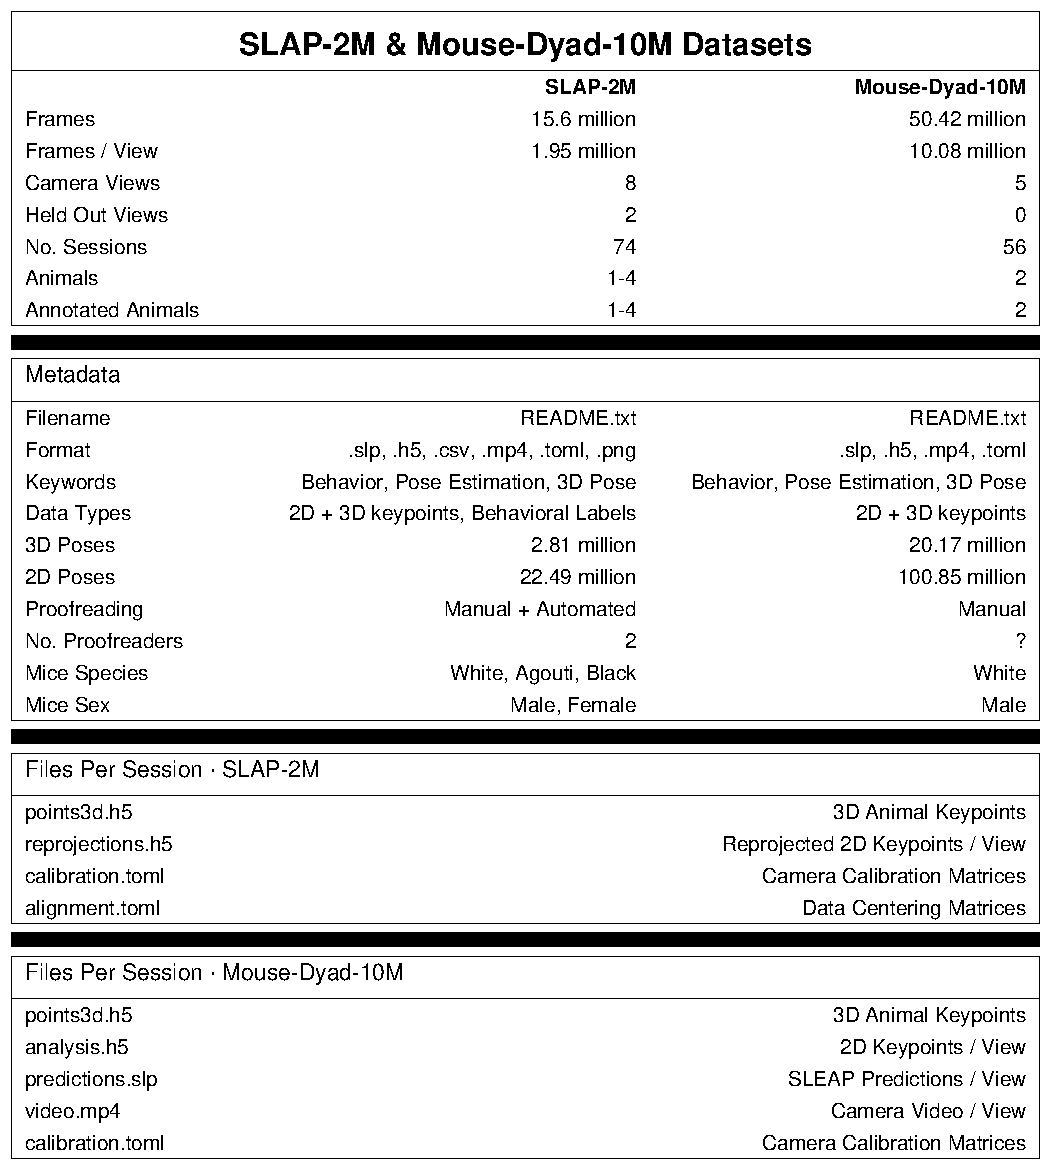
\includegraphics[width=0.95\textwidth]{figs/datasheet_combined.pdf}
  \captionsetup{font=scriptsize}
  \captionof{table}{\textbf{Dataset datasheets.} Composition, metadata and per-session file inventory of the two corpora. SLAP-2M: 74 sessions, 8 camera views (2 held out from proofreading), 1--4 animals. Mouse-Dyad-10M: 56 sessions, 5 camera views, 2 animals, 10.08 million frames per view. 2D pose counts are reprojections of the 3D poses into every view.}
  \label{tab:datasheets}
\end{figure}

\FloatBarrier

\begin{thebibliography}{99}

\bibitem{Aldarondo2019} Aldarondo, D. (2019). Label3D. https://github.com/diegoaldarondo/Label3D

\bibitem{Aharon2026} Aharon, L., Whiteway, M. R., Sikka, K., Lee, K., Wang, Y., Chettih, S., et al. (2026). Lightning Pose 3D: an uncertainty-aware framework for data-efficient multi-view animal pose estimation. \textit{bioRxiv}.

\bibitem{Bernardin2008} Bernardin, K., \& Stiefelhagen, R. (2008). Evaluating multiple object tracking performance: The CLEAR MOT metrics. \textit{EURASIP Journal on Image and Video Processing}, 2008, 246309.

\bibitem{Biderman2024} Biderman, D., Whiteway, M. R., Hurwitz, C., Greenspan, N., Lee, R. S., Vishnubhotla, A., et al. (2024). Lightning Pose: improved animal pose estimation via semi-supervised learning, Bayesian ensembling and cloud-native open-source tools. \textit{Nature Methods}, 21(7), 1316--1328.

\bibitem{Chen2020} Chen, L., Ai, H., Chen, R., Zhuang, Z., \& Liu, S. (2020). Cross-view tracking for multi-human 3D pose estimation at over 100 FPS. In \textit{Proceedings of the IEEE/CVF Conference on Computer Vision and Pattern Recognition (CVPR)}, 3276--3285.

\bibitem{Daruwalla2026} Daruwalla, K., Nozal Martin, I., Zhang, L., Naglič, D., Frankel, A., Rasgaitis, C., et al. (2026). Cheese3D enables sensitive detection and analysis of whole-face movement in mice. \textit{Nature Neuroscience}, 1--12.

\bibitem{Dias2025} Dias, I. C., Gutierrez-Castellanos, N., Lenschow, C., \& Lima, S. Q. (2025). Ready or not: Neural mechanisms regulating female sexual behavior. \textit{Current Opinion in Neurobiology}, 93, 103069.

\bibitem{Dunn2021} Dunn, T. W., et al. (2021). Geometric deep learning enables 3D kinematic profiling across species and environments. \textit{Nature Methods}, 18, 564--573.

\bibitem{Huang2020} Huang, C., Jiang, S., Li, Y., Zhang, Z., Traish, J., Deng, C., et al. (2020). End-to-end dynamic matching network for multi-view multi-person 3D pose estimation. In \textit{European Conference on Computer Vision}, 477--493. Cham: Springer International Publishing.

\bibitem{Heindl2024} Heindl, C., Valmadre, J., et al. (2024). py-motmetrics: Benchmark multiple object trackers (MOT) in Python (v1.4.0). \textit{Zenodo}. https://doi.org/10.5281/zenodo.14014773

\bibitem{Hueser2023} Hueser, T. (2023). JARVIS Annotation Tool. https://github.com/JARVIS-MoCap/JARVIS-AnnotationTool

\bibitem{Iskakov2019} Iskakov, K., Burkov, E., Lempitsky, V., \& Malkov, Y. (2019). Learnable Triangulation of Human Pose. In \textit{Proceedings of the IEEE/CVF International Conference on Computer Vision (ICCV)}, 7718--7727.

\bibitem{Klibaite2025} Klibaite, U., Li, T., Aldarondo, D., Akoad, J. F., Ölveczky, B. P., \& Dunn, T. W. (2025). Mapping the landscape of social behavior. \textit{Cell}, 188(8), 2249--2266.

\bibitem{Karashchuk2021} Karashchuk, P., Rupp, K. L., Dickinson, E. S., Walling-Bell, S., Sanders, E., Azim, E., Brunton, B. W., \& Tuthill, J. C. (2021). Anipose: A toolkit for robust markerless 3D pose estimation. \textit{Cell Reports}, 36(13), 109730.

\bibitem{Lever2006} Lever, C., Burton, S., \& O Keefe, J. (2006).  Rearing on hind legs, environmental novelty, and the hippocampal formation. \textit{Reviews in the Neurosciences}, 17(1/2), 111.

\bibitem{Leonardis2022} Leonardis, E. J., Breston, L., Lucero-Moore, R., Sena, L., Kohli, R., Schuster, L., Barton-Gluzman, L., Quinn,  L. K., Wiles, J., \& Chiba, A. A. (2022). Interactive neurorobotics: Behavioral and neural dynamics of agent interactions. \textit{Frontiers in Psychology}, 13, 897603.

\bibitem{Leonardis2025} Leonardis, E., Nagamori, A., Thanawalla, A., Yang, Y., Park, J., Saunders, H., et al. (2025). Massively Parallel Imitation Learning of Mouse Forelimb Musculoskeletal Reaching Dynamics. \textit{arXiv:2511}.

\bibitem{Maree2024} Maree, L., Afshar, S., Oline, S., Leonardis, E. J., Falkner, A. L., \& Pereira, T. D. (2024). Multi-view triangulation-enabled annotation for multi-animal 3D pose in SLEAP. In \textit{Measuring Behavior}.

\bibitem{Marshall2021} Marshall, J. D., Klibaite, U., Gellis, A., Aldarondo, D. E., Ölveczky, B. P., \& Dunn, T. W. (2021). The PAIR-R24M Dataset for Multi-animal 3D Pose Estimation. \textit{bioRxiv}, 2021.11.23.469743.

\bibitem{Marshall2022} Marshall, J. D., Li, T., Wu, J. H., \& Dunn, T. W. (2022). Leaving flatland: Advances in 3D behavioral measurement. \textit{Current Opinion in Neurobiology}, 73, 102522.

\bibitem{Mathis2018} Mathis, A., Mamidanna, P., Cury, K. M., Abe, T., Murthy, V. N., Mathis, M. W., \& Bethge, M. (2018). DeepLabCut: markerless pose estimation of user-defined body parts with deep learning. \textit{Nature Neuroscience}, 21(9), 1281--1289.

\bibitem{Pereira2020} Pereira, T. D., Shaevitz, J. W., \& Murthy, M. (2020). Quantifying behavior to understand the brain. \textit{Nature Neuroscience}, 23(12), 1537--1549.

\bibitem{Pereira2022} Pereira, T. D., Tabris, N., Matsliah, A., Turner, D. M., Li, J., Ravindranath, S., et al. (2022). SLEAP: A deep learning system for multi-animal pose tracking. \textit{Nature Methods}, 19(4), 486--495.

\bibitem{Ristani2016} Ristani, E., Solera, F., Zou, R., Cucchiara, R., \& Tomasi, C. (2016). Performance measures and a data set for multi-target, multi-camera tracking. In \textit{European Conference on Computer Vision Workshops} (pp. 17--35). Springer.

\bibitem{Waldmann2024} Waldmann, U., Chan, A. H. H., Naik, H., Nagy, M., Couzin, I. D., Deussen, O., ... \& Kano, F. (2024). 3d-muppet: 3d multi-pigeon pose estimation and tracking. \textit{International Journal of Computer Vision}, 132(10), 4235-4252.

\bibitem{Zhang2025} Zhang, C. Y., Yang, Y., Sirbu, A., Abe, E. T., Wärnberg, E., Leonardis, E. J., et al. (2025). MIMIC-MJX: Neuromechanical emulation of animal behavior. \textit{arXiv:2511}.

\end{thebibliography}


\end{document}